\chapter{Development of the Integration Pipeline}
\label{ch:execution}

This chapter describes the development and execution of each stage of the integration pipeline designed in Chapter~\ref{ch:solution-design}. The presentation follows the chronological order in which the work was carried out: first, the exploratory analysis of the original datasets; then, the examination of the MIOTTA-NPT processed versions; and finally, the execution of the integration pipeline that produces the unified dataset.

% ══════════════════════════════════════════════════════════════════════════════
\section{Exploratory Analysis of Original Datasets}
\label{sec:eda-original}

Before proceeding with the integration, each dataset was subjected to comprehensive exploratory data analysis in its original feature representation. This step served to understand the structure, content, and quality of each source, and to identify characteristics that would inform the subsequent integration decisions.

\subsection{CICIoMT2024 --- Original Feature Space}
\label{subsec:eda-ciciomt}

The CICIoMT2024 dataset, introduced by Dadkhah et al.~\cite{dadkhah2024ciciomt}, was created by the Canadian Institute for Cybersecurity specifically for evaluating the security of IoMT devices. The experimental testbed comprised 40 IoMT devices (25 real and 15 simulated via IoTFlock), with attacks executed by four Raspberry Pi units across WiFi and MQTT protocols. Features were extracted from raw PCAP files using a DPKT-based window aggregation pipeline---the same extraction methodology employed for CICIoT2023.

The exploratory analysis revealed the following characteristics:

\begin{itemize}
    \item \textbf{Scale}: 8,322,896 records (6,708,714 training, 1,614,182 test), each described by 45 features. The dataset occupies approximately 5.1~GB in memory.
    \item \textbf{Feature space}: All 45 features are numeric (\texttt{float64}), comprising packet/flow statistics (Header\_Length, Rate, Tot\_size, IAT), protocol indicator flags (HTTP, DNS, TCP, UDP, MQTT), and TCP flag counts. Notably, the \texttt{Duration} column actually encodes TTL (Time-To-Live) values (range 0--255), not time duration---a critical observation for correct interpretation.
    \item \textbf{Attack taxonomy}: 18 distinct attack types organized into 5 categories---DDoS (4~types, 66.6\%), DoS (4~types, 26.7\%), MQTT (5~types, 3.3\%), Reconnaissance (4~types, 1.6\%), and Spoofing (1~type, 0.2\%)---plus Benign traffic (1.6\%). The 5 MQTT-specific attacks (DDoS/DoS Connect and Publish Flood, Malformed Data) are unique to this dataset and not present in CICIoT2023.
    \item \textbf{Class imbalance}: Substantial, with a maximum-to-minimum ratio of approximately 2,157:1 between DDoS variants and Spoofing. At the binary level, attack traffic constitutes 98.4\% of records.
    \item \textbf{Data quality}: Minimal issues---only 148 missing values (in the Weight and Variance features), no infinite values, and 7,216 duplicate rows (0.09\%).
\end{itemize}

\subsection{IoMT-TrafficData --- Original Feature Space}
\label{subsec:eda-iomt-traffic}

The IoMT-TrafficData dataset, introduced by Areia et al.~\cite{areia2024iomt}, provides network traffic from a hospital-oriented IoMT testbed with 10+ medical devices communicating over CoAP, MQTT, and HTTP protocols. Unlike the CIC datasets, features were extracted using \textbf{Zeek} (formerly Bro), a flow-oriented network analysis framework that produces per-connection records rather than window-based aggregations.

The exploratory analysis revealed characteristics fundamentally different from CICIoMT2024:

\begin{itemize}
    \item \textbf{Scale}: 969,141 flow records described by 101 features (88 numeric, 13 categorical/string). The dataset is considerably smaller than CICIoMT2024 but provides complementary attack coverage.
    \item \textbf{Feature space}: The 101 Zeek-derived features are organized into functional groups---connection metadata (15 features), Zeek base statistics (6), flow duration and rates (6), forward packet statistics (20), backward packet statistics (20), flow-level packet statistics (11), inter-arrival times (7), active/idle periods (4), bulk transfer metrics (6), and TCP window sizes (6). This schema is semantically richer than the CIC window-based features but structurally incompatible: direct column-matching between the two schemas is not possible.
    \item \textbf{Attack taxonomy}: 8 attack types plus Benign traffic---ARP Spoofing, Apache Killer (DoS), CAM Table Overflow, MQTT Malaria (MQTT flooding), Reconnaissance (Netscan), R-U-Dead-Yet/RUDY (slow POST), Slow Loris (slow HTTP), and Slow Read (slow read DoS). Several of these overlap with CICIoMT2024 attacks (ARP Spoofing, Reconnaissance, DoS variants), enabling cross-dataset label harmonization.
    \item \textbf{Class imbalance}: Moderate, with a maximum-to-minimum ratio of approximately 22:1---significantly less extreme than CICIoT2023 but still requiring attention during model training.
    \item \textbf{Data quality}: No missing values and no infinite values in the original data. However, 8 features exhibited zero variance and 17 had near-zero variance (>95\% identical values), indicating that a substantial portion of the feature space carries minimal discriminative information. Additionally, 36 features showed high skewness ($|s| > 5$), and 6,434 duplicate rows (0.66\%) were identified.
    \item \textbf{Integration implication}: The fundamental difference between the Zeek flow-level schema and the DPKT window-based schema used by the CIC datasets confirmed that semantic feature mapping alone would be insufficient for reliable integration. This observation was a primary motivation for adopting MIOTTA-NPT as the unifying feature extraction tool, as it can reprocess the raw PCAPs from all datasets into a common representation.
\end{itemize}

\subsection{CICIoT2023 --- Original Feature Space}
\label{subsec:eda-ciciot}

The CICIoT2023 dataset, introduced by Neto et al.~\cite{neto2023ciciot2023}, represents the largest-scale IoT attack dataset employed in this work. It was generated in a realistic smart-home topology comprising 105 IoT devices (67 directly involved, 38 Zigbee/Z-Wave peripherals), with 7 Raspberry Pi units orchestrating attacks. Feature extraction followed the same DPKT window-based aggregation pipeline as CICIoMT2024, establishing structural compatibility between the two CIC datasets.

The exploratory analysis revealed:

\begin{itemize}
    \item \textbf{Scale}: 44,763,144 records distributed across 63 CSV files (\(\sim\)9.1~GB), each record described by 39 features plus a label column (40 columns total). This makes it the largest dataset by an order of magnitude.
    \item \textbf{Feature space}: 39 features---38 \texttt{float64} and 1 \texttt{int64} (Protocol Type). The feature set largely overlaps with CICIoMT2024 (same extraction methodology), although 7 features documented in the paper (including \texttt{flow\_duration}, \texttt{Srate}, \texttt{Drate}, \texttt{urg\_count}, \texttt{Magnitue}, \texttt{Radius}, \texttt{Covariance}) are absent from the actual CSV files, while \texttt{IGMP} and \texttt{Time\_To\_Live} appear as extras. This discrepancy between the published schema and the distributed data was an important finding.
    \item \textbf{Attack taxonomy}: 33 distinct attack types organized into 7 categories---DDoS (12~types, \(\sim\)34M records), DoS (4~types, \(\sim\)8.1M), Mirai (3~types, \(\sim\)2.6M), Benign (\(\sim\)1.1M), Spoofing (2~types, \(\sim\)0.5M), Reconnaissance (5~types, \(\sim\)0.35M), Web-based (6~types, \(\sim\)25K), and Brute Force (1~type, \(\sim\)13K). The Mirai, Web-based, and Brute Force categories are exclusive to this dataset and not found in the IoMT-specific sources.
    \item \textbf{Class imbalance}: Extreme, with a maximum-to-minimum ratio of approximately 5,750:1 between DDOS-ICMP\_FLOOD (6.85M records) and UPLOADING\_ATTACK (1,192 records). At the binary level, 97.7\% of records represent attack traffic.
    \item \textbf{Data quality}: 35 infinity values (concentrated in the Rate feature, replaced with NaN), 1,803,394 missing values after replacement, and a high duplicate rate of 33.33\% in the analyzed sample. The elevated duplication is attributable to the window-based aggregation methodology, where consecutive windows of identical packet patterns produce identical feature vectors.
    \item \textbf{Window aggregation bias}: Different attack categories use different window sizes---10 packets for low-volume attacks (Web-based, Reconnaissance, Spoofing, Benign, Brute Force) and 100 packets for high-volume attacks (DDoS, DoS, Mirai). This introduces a systematic methodological difference across categories that must be considered when interpreting per-category results.
\end{itemize}

\subsection{Key Observations from Original Analyses}
\label{subsec:eda-summary}

A critical finding from the exploratory analyses is the fundamental structural incompatibility across the three datasets. As illustrated in Figure~\ref{fig:feature-count-comparison}, each dataset was originally extracted using a different tool and yields a different number of features: CICIoMT2024 provides 45 features (CIC internal tool), IoMT-TrafficData provides 101 features (Zeek), and CICIoT2023 provides 47 features (CIC internal tool). Beyond the numerical difference, the features carry different semantics---Zeek operates at the flow level with a distinct aggregation logic compared to the CIC window-based approach. This incompatibility confirmed the necessity of re-extracting all datasets through MIOTTA-NPT to achieve a unified feature space.

\begin{figure}[htbp]
\centering
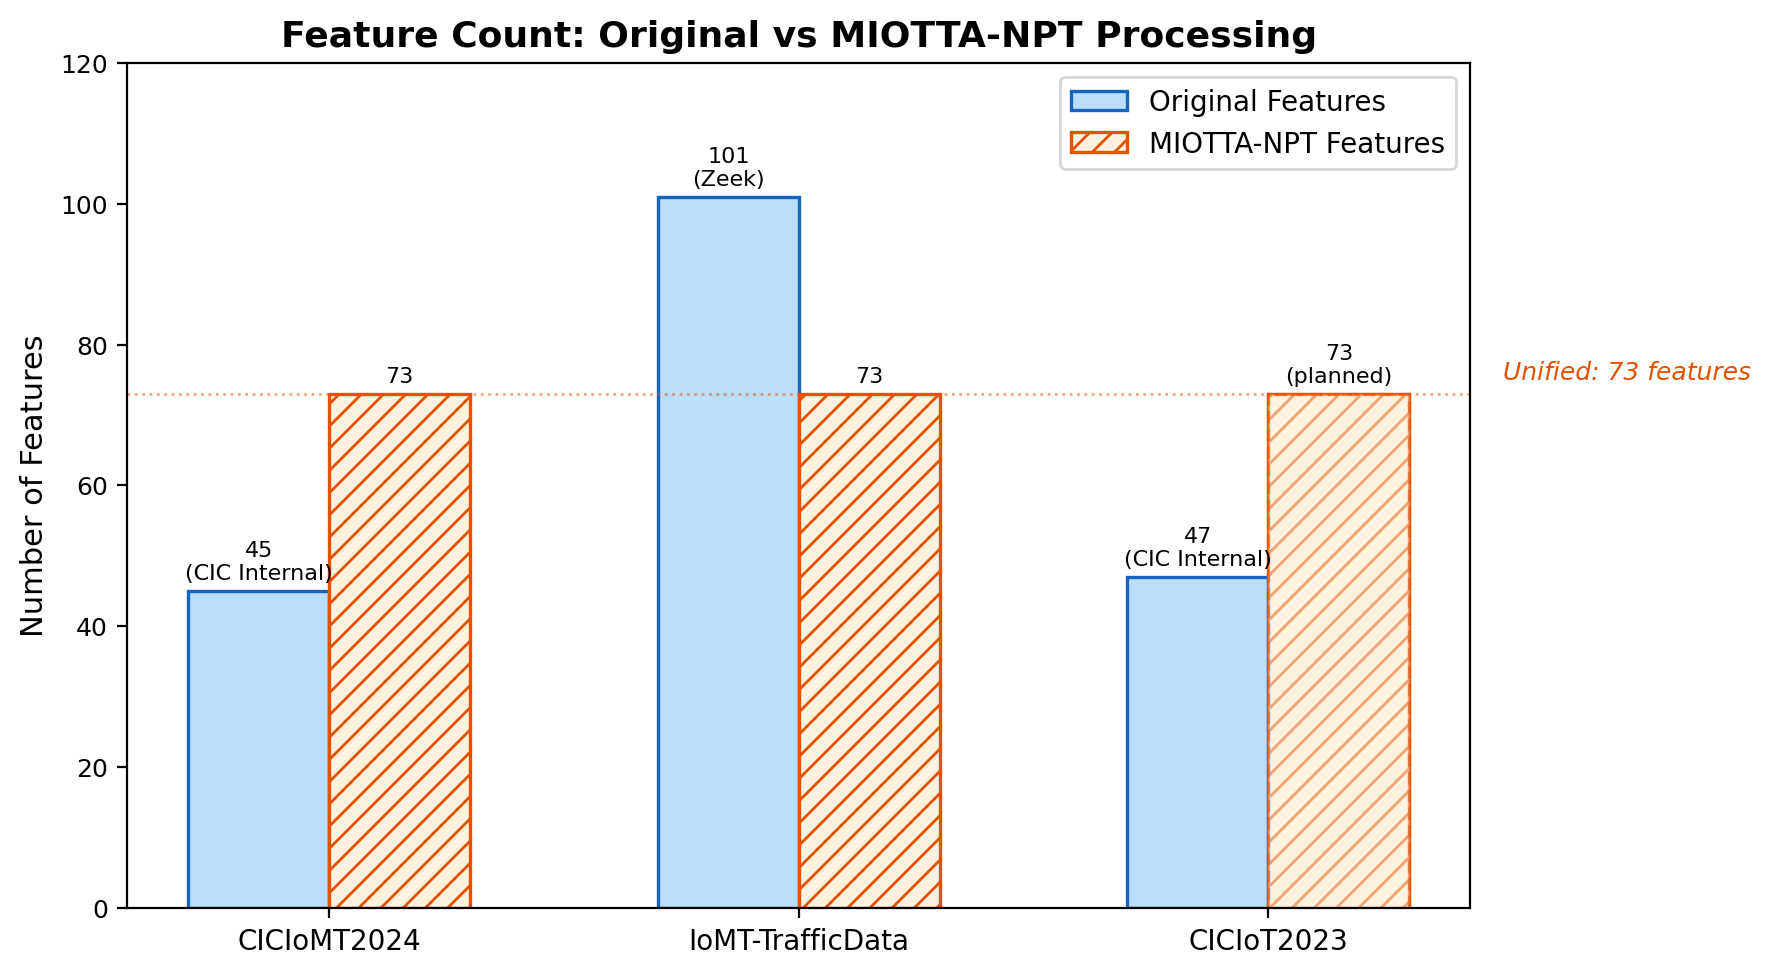
\includegraphics[width=0.85\textwidth]{feature_count_comparison.png}
\caption{Comparison of original feature counts across the three datasets versus the standardized 73-feature space produced by MIOTTA-NPT. The dashed bar for CICIoT2023 indicates that its MIOTTA-NPT processing is planned for Phase~2. The horizontal dotted line marks the unified target of 73 features.}
\label{fig:feature-count-comparison}
\end{figure}

% ══════════════════════════════════════════════════════════════════════════════
\section{MIOTTA-NPT Feature Extraction Results}
\label{sec:miotta-results}

This section presents the results of processing the available datasets through MIOTTA-NPT, verifying that the tool produces the expected standardized feature space and examining the characteristics of the resulting data. Figure~\ref{fig:dataset-summary} provides an overview of the two MIOTTA-processed datasets.

\begin{figure}[htbp]
\centering
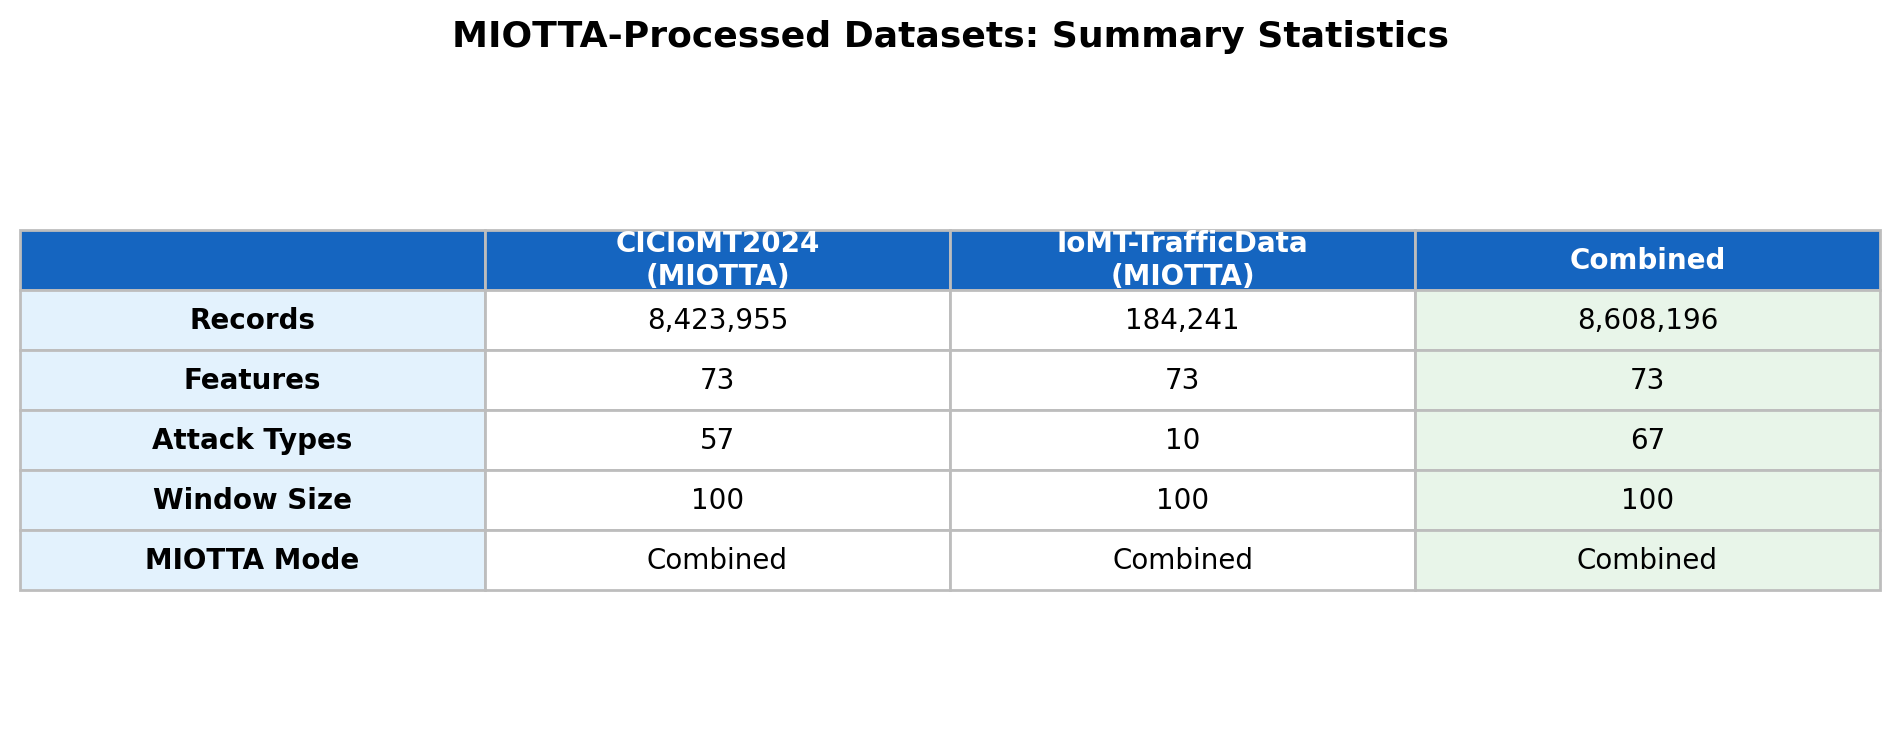
\includegraphics[width=0.85\textwidth]{dataset_summary_table.png}
\caption{Summary statistics of the two MIOTTA-processed datasets. Both datasets share an identical 73-feature space extracted in combined mode with a window size of 100 packets.}
\label{fig:dataset-summary}
\end{figure}

\subsection{CICIoMT2024 --- MIOTTA-Processed}
\label{subsec:miotta-ciciomt}

The MIOTTA-NPT processing of CICIoMT2024 yielded 8,423,955 records (6,872,287 train and 1,551,668 test) across 73 features, covering all 18 original attack types plus benign traffic. Figure~\ref{fig:ciciomt-attack-dist} shows the distribution of records across attack types, revealing significant class imbalance---a characteristic inherited from the original dataset that the integration pipeline must address.

\begin{figure}[htbp]
\centering
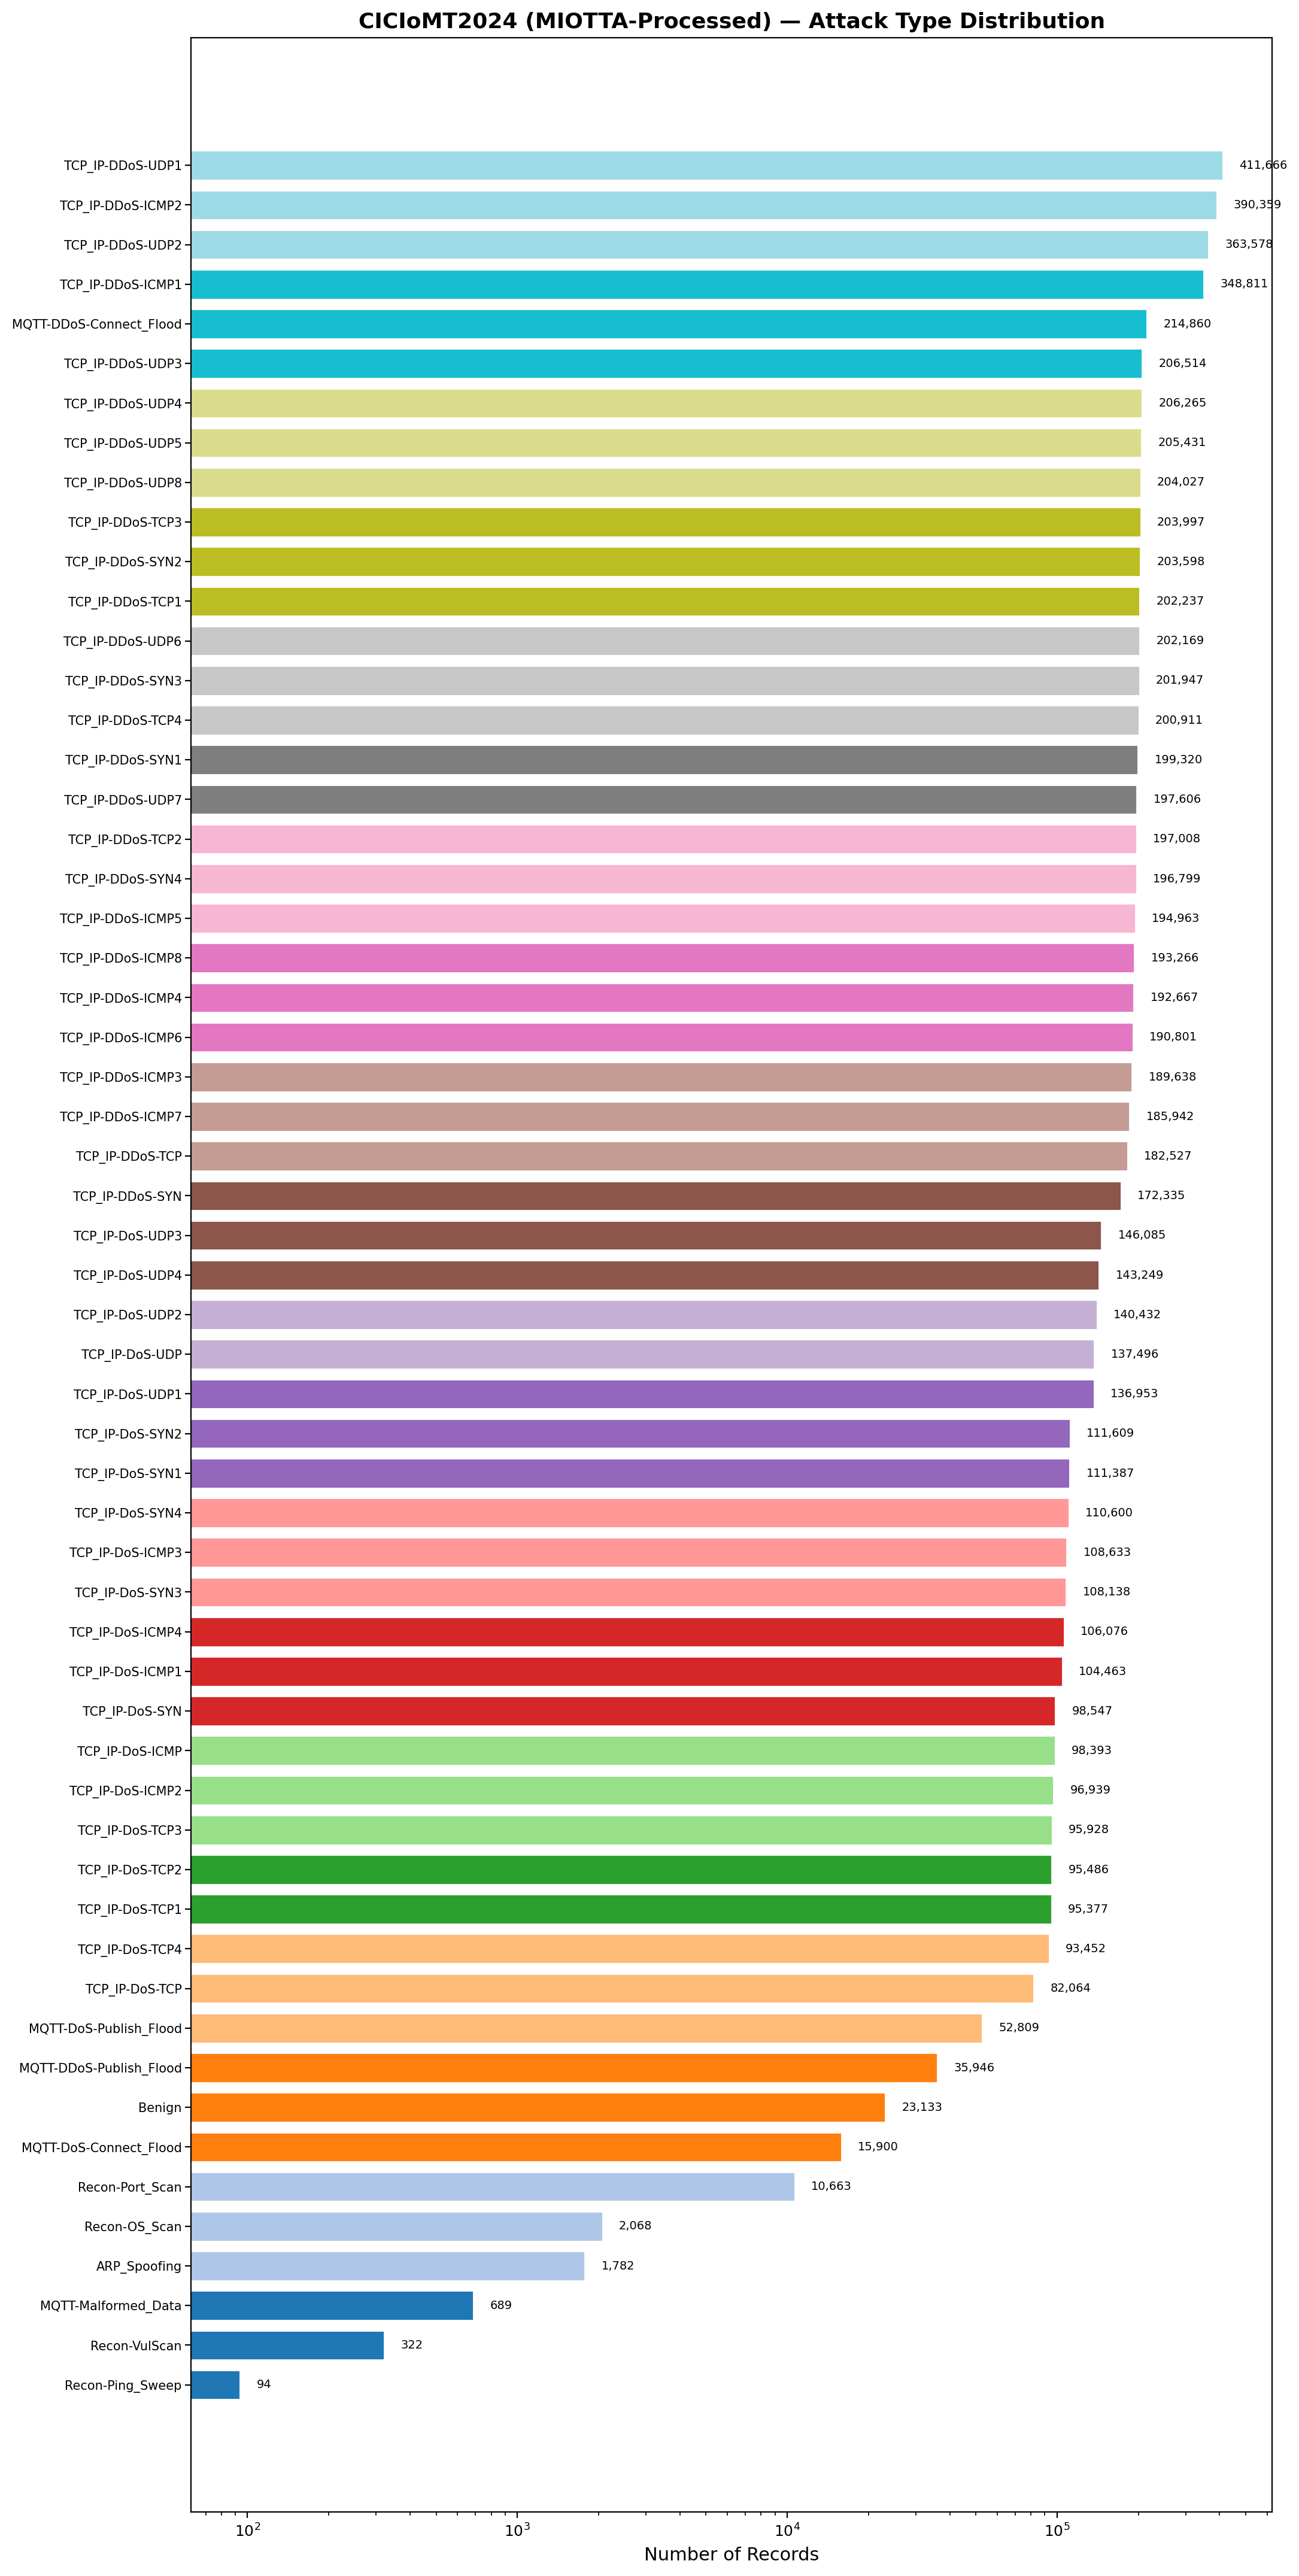
\includegraphics[height=0.86\textheight, keepaspectratio]{ciciomt2024_miotta_attack_dist.png}
\caption{Attack type distribution in the MIOTTA-processed CICIoMT2024 dataset. The logarithmic scale reveals the substantial class imbalance, with certain attack types (e.g., DDoS variants) having orders of magnitude more records than others.}
\label{fig:ciciomt-attack-dist}
\end{figure}

\subsection{IoMT-TrafficData --- MIOTTA-Processed}
\label{subsec:miotta-iomt-traffic}

The MIOTTA-NPT processing of IoMT-TrafficData produced 184,241 records across the same 73 features. Figure~\ref{fig:iomt-attack-dist} shows the attack type distribution. Compared to CICIoMT2024, this dataset is considerably smaller but provides complementary attack coverage, particularly in categories such as Apache Killer, CAM Table Overflow, and RUDY that are not present in CICIoMT2024.

\begin{figure}[htbp]
\centering
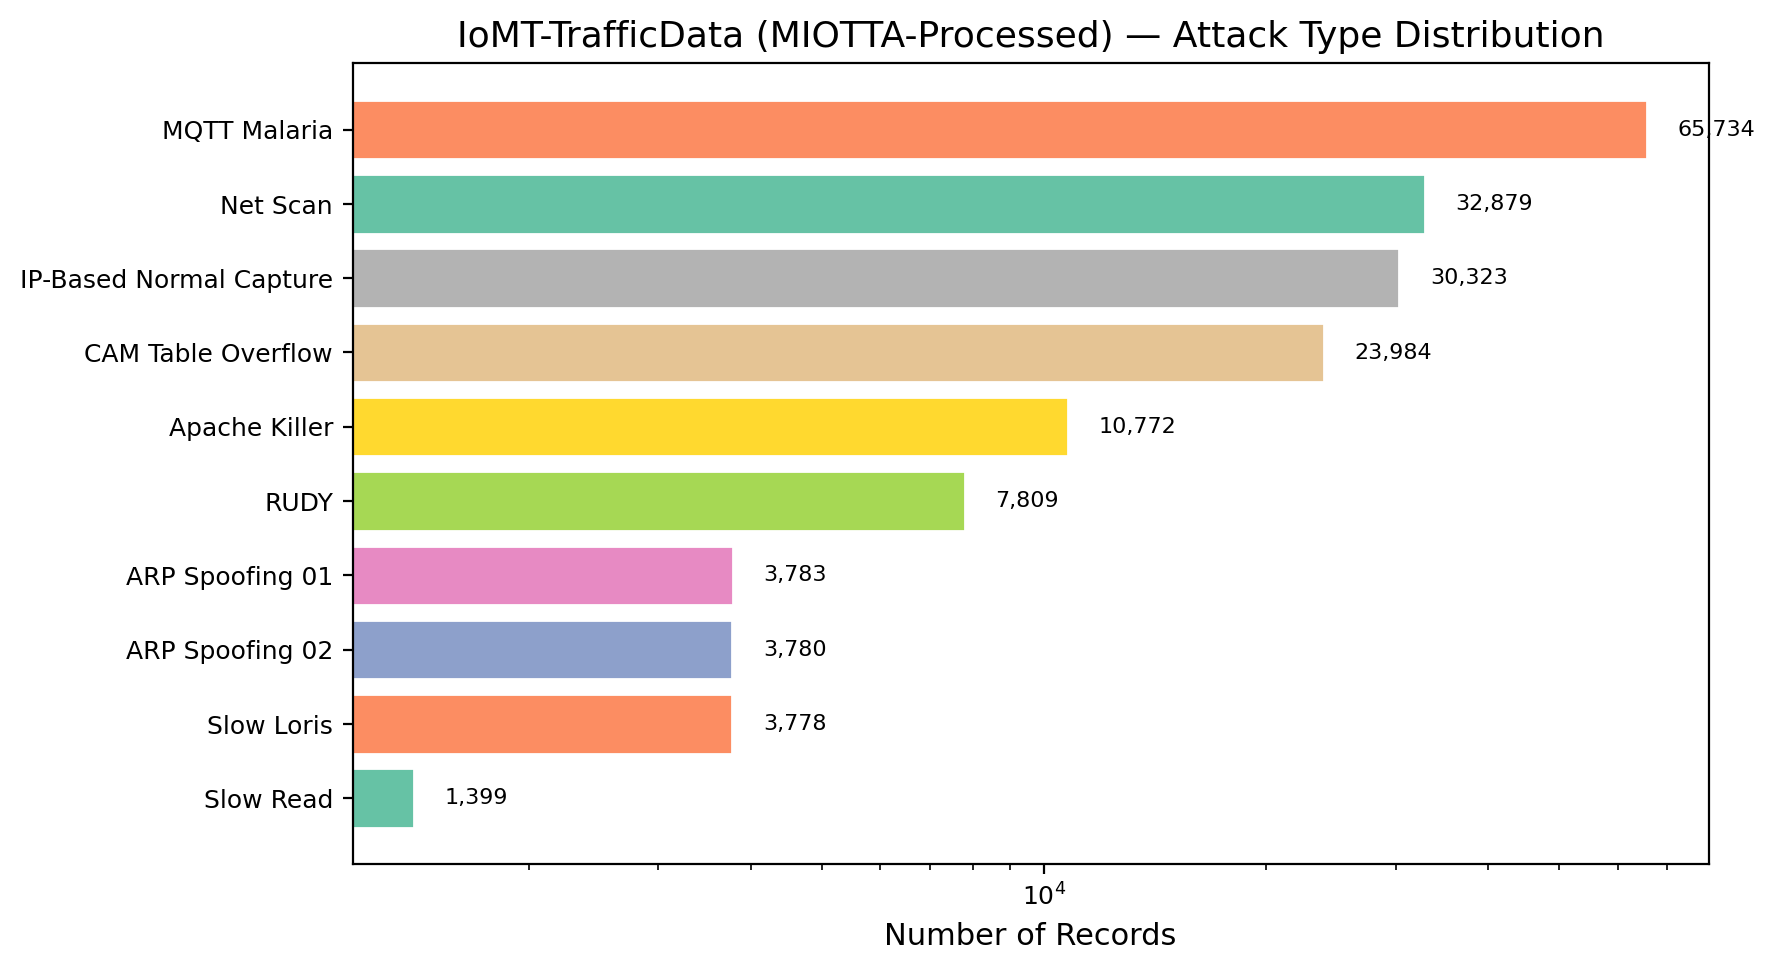
\includegraphics[width=0.85\textwidth]{iomt_traffic_miotta_attack_dist.png}
\caption{Attack type distribution in the MIOTTA-processed IoMT-TrafficData dataset. The dataset contains 10 traffic categories including benign traffic and 9 attack types relevant to IoMT environments.}
\label{fig:iomt-attack-dist}
\end{figure}

\subsection{Cross-Dataset Feature Verification}
\label{subsec:feature-verification}

A fundamental prerequisite for the integration is that both MIOTTA-processed datasets share an identical feature space. This was verified empirically, as shown in Figure~\ref{fig:feature-verification}: both datasets produce exactly 73 columns with identical names and data types, confirming that MIOTTA-NPT resolves the feature heterogeneity problem at the source.

\begin{figure}[htbp]
\centering
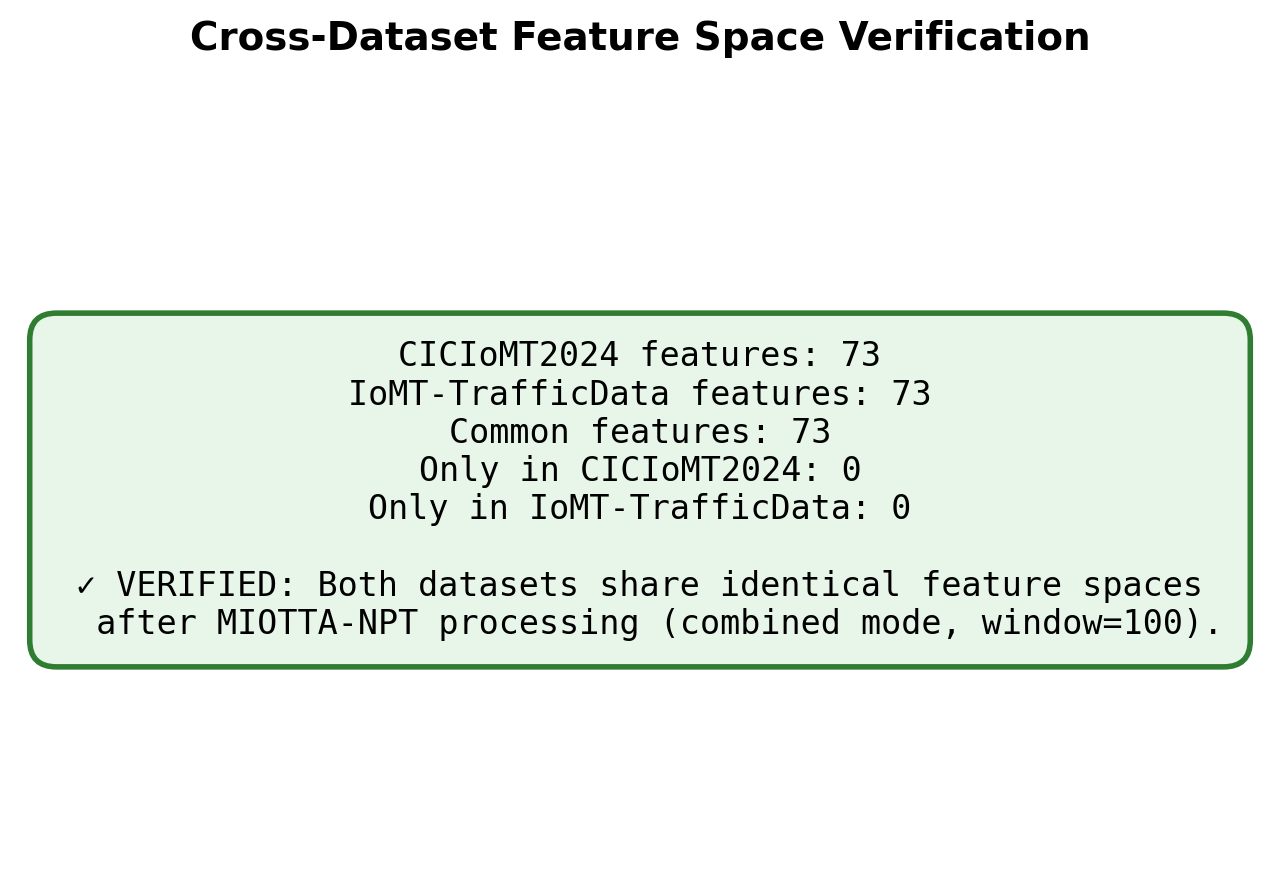
\includegraphics[width=0.7\textwidth]{feature_verification.png}
\caption{Cross-dataset feature space verification. The comparison confirms that both MIOTTA-processed datasets share an identical set of 73 features, with no dataset-exclusive columns.}
\label{fig:feature-verification}
\end{figure}

While the feature names are identical, the value distributions differ across datasets---reflecting genuine differences in network traffic characteristics. Figure~\ref{fig:feature-distributions} presents the distributions of eight key features across both datasets, revealing notable differences in value ranges and distribution shapes. These differences are expected and desirable, as they represent the diversity of network environments that the unified dataset aims to capture.

\begin{figure}[htbp]
\centering
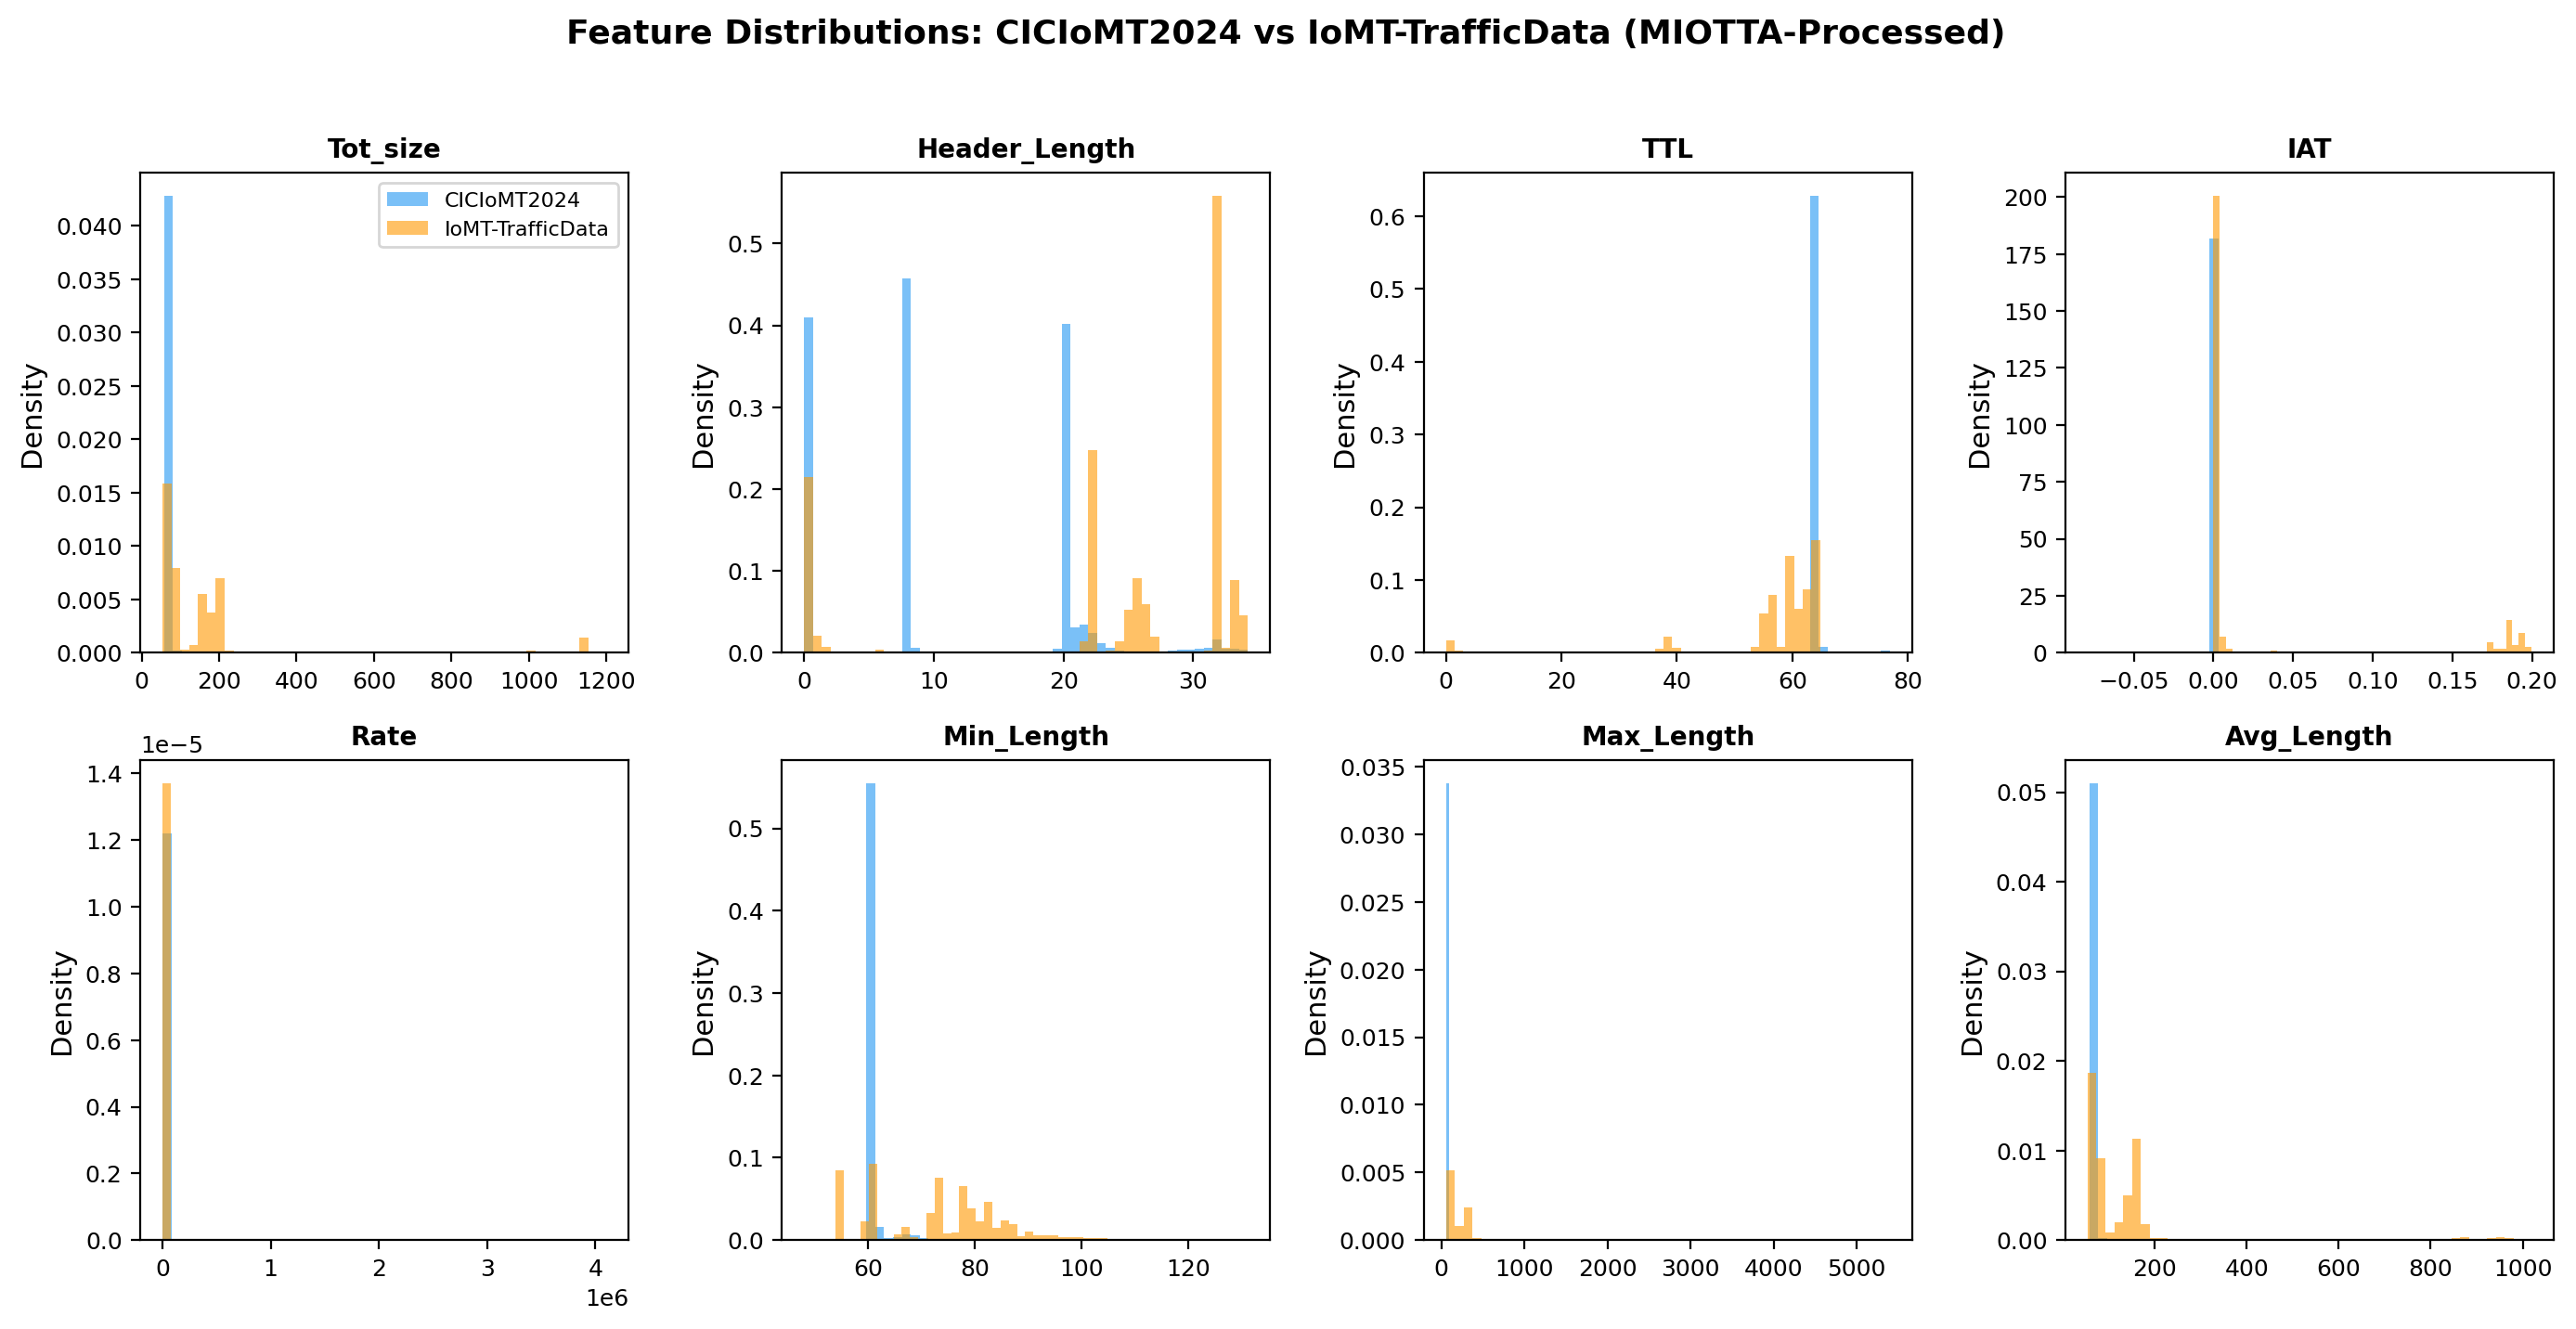
\includegraphics[width=\textwidth]{feature_distributions_comparison.png}
\caption{Distribution comparison of key features across the two MIOTTA-processed datasets (99th percentile clipping applied for visualization). The differences in distributions reflect genuine variation in network traffic characteristics between the two environments.}
\label{fig:feature-distributions}
\end{figure}

The correlation structure of the features was also examined. Figure~\ref{fig:correlation-heatmaps} shows the correlation matrices for both datasets, revealing similar overall patterns but with notable differences in the strength of certain inter-feature correlations. Several feature groups exhibit high mutual correlation (e.g., forward/backward packet statistics), which is consistent with the nature of network traffic data.

\begin{figure}[htbp]
\centering
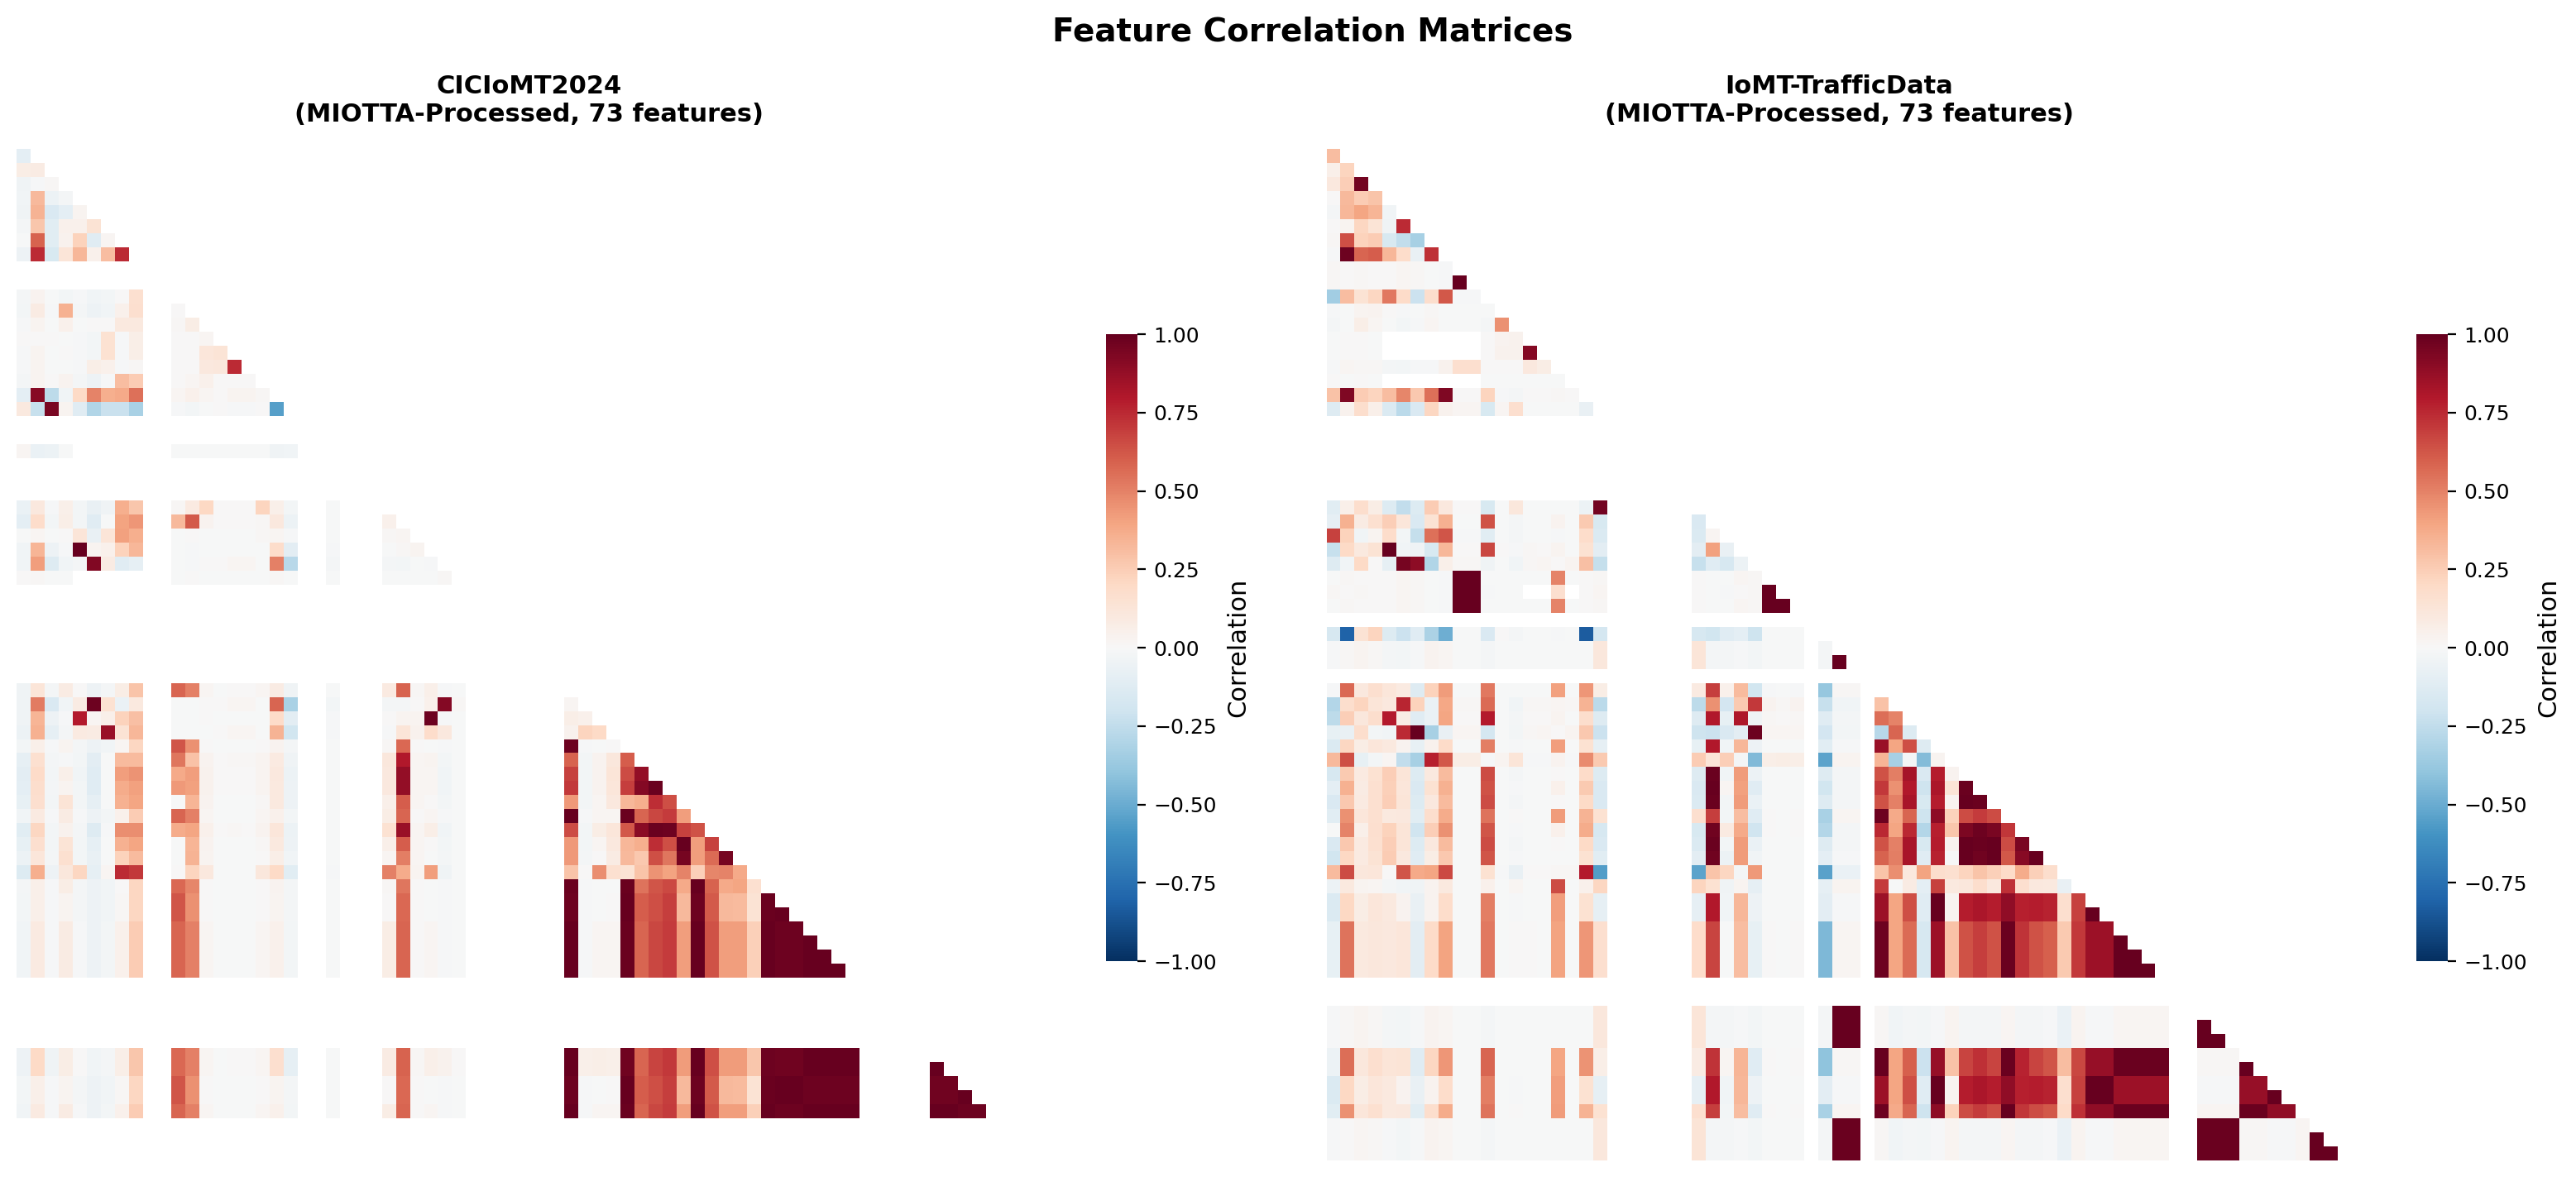
\includegraphics[width=\textwidth]{correlation_heatmaps.png}
\caption{Feature correlation matrices for CICIoMT2024 (left) and IoMT-TrafficData (right), both MIOTTA-processed. Similar overall correlation patterns are observed, with clusters of highly correlated features in the packet statistics and TCP flag groups.}
\label{fig:correlation-heatmaps}
\end{figure}

The analysis of missing values, presented in Figure~\ref{fig:missing-values}, reveals that certain features (primarily TCP flag statistics) contain NaN values. This is expected behavior: windows that contain only non-TCP traffic (e.g., purely ARP or UDP traffic) naturally lack TCP flag statistics. The integration pipeline addresses this through targeted imputation with zero values for protocol-absent features.

\begin{figure}[htbp]
\centering
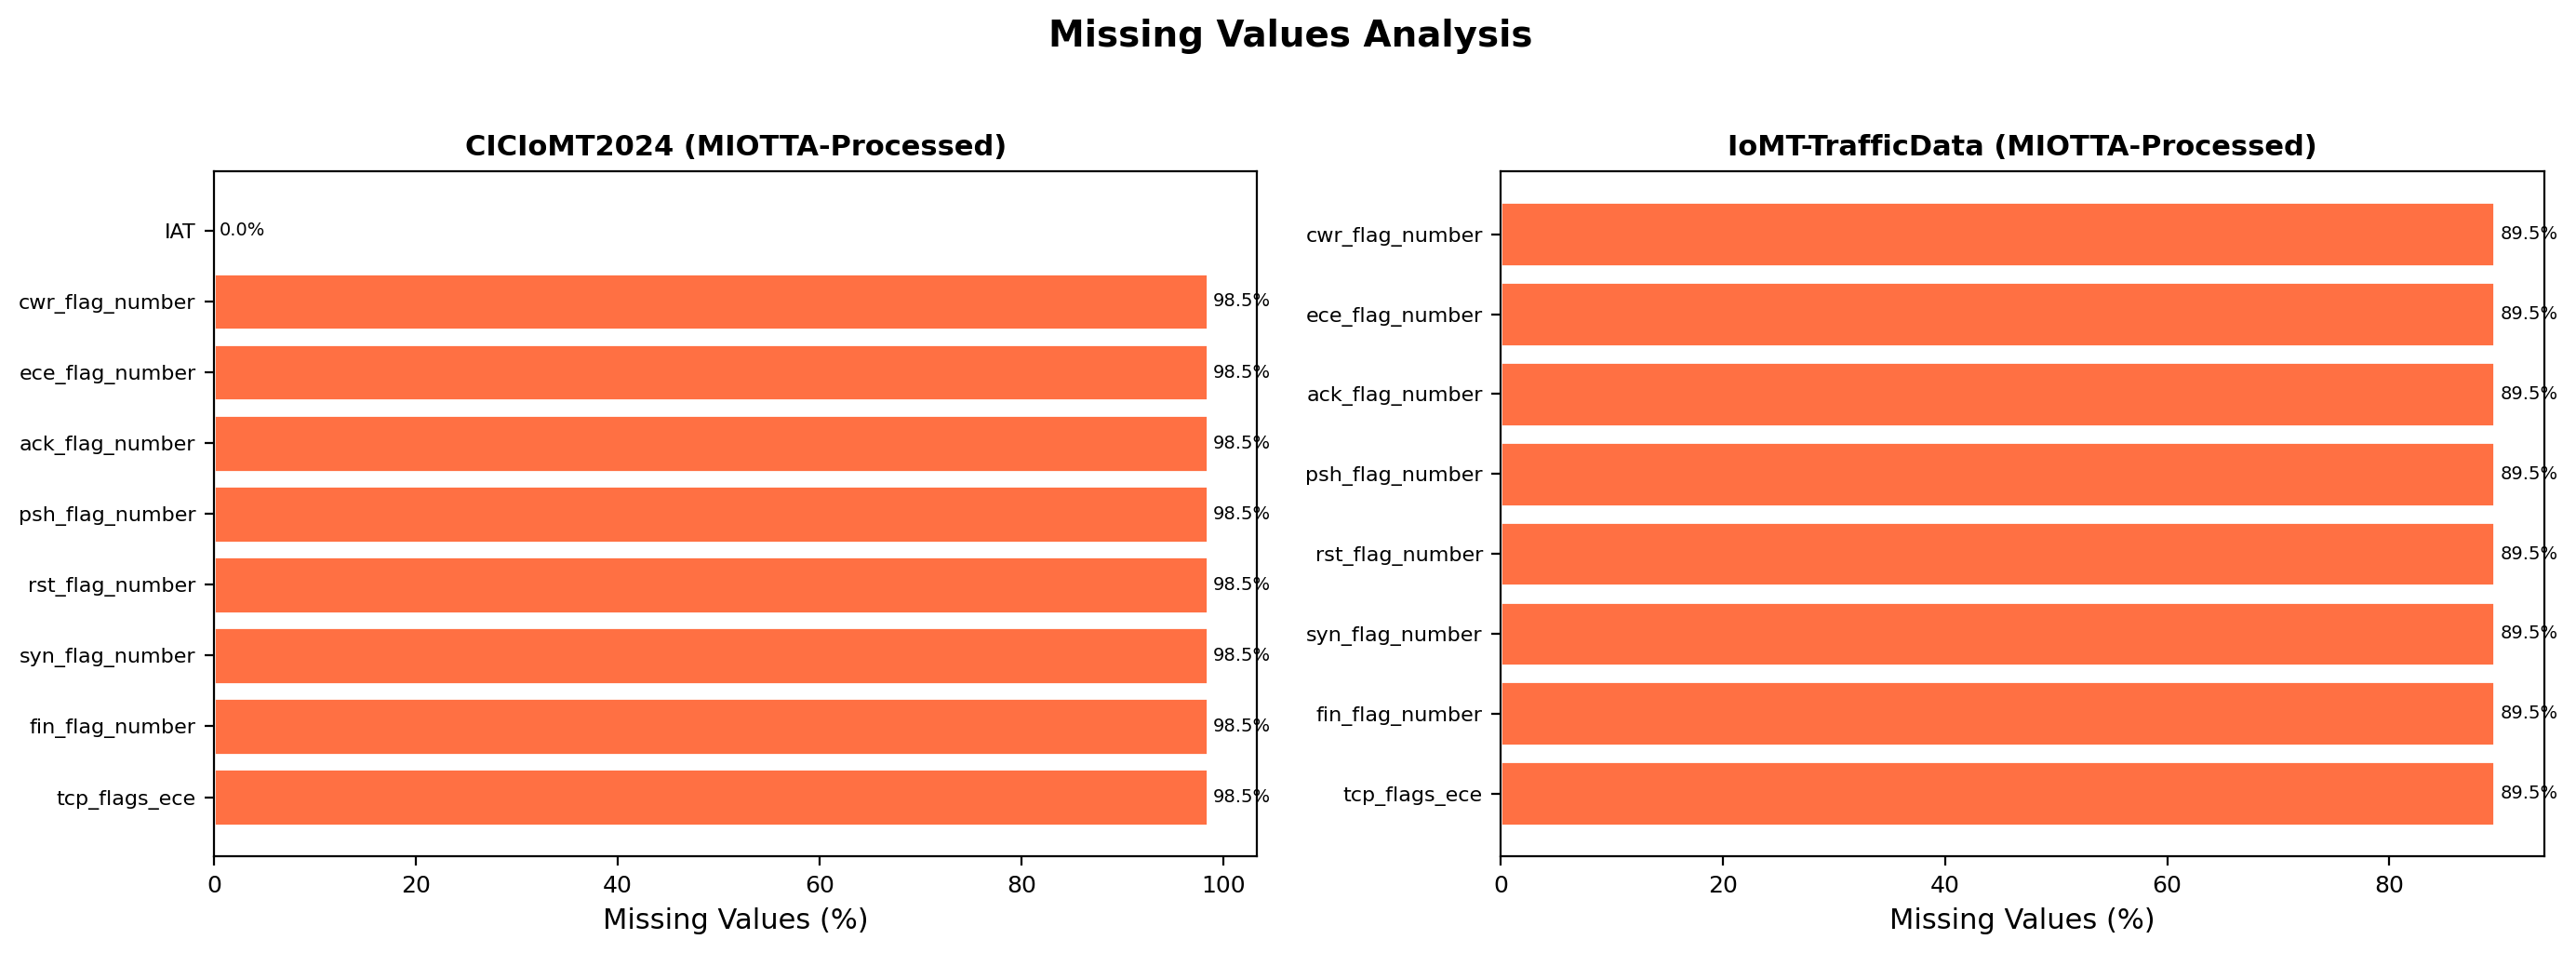
\includegraphics[width=\textwidth]{missing_values_analysis.png}
\caption{Missing values analysis for both MIOTTA-processed datasets. NaN values are concentrated in TCP flag features and arise from windows containing only non-TCP traffic---an expected and well-understood pattern.}
\label{fig:missing-values}
\end{figure}

\subsection{CICIoT2023 --- Planned MIOTTA Processing}
\label{subsec:miotta-ciciot-planned}

The CICIoT2023 dataset will be processed through MIOTTA-NPT using the same configuration (combined mode, window size of 100 packets) as part of Phase~2. Based on the verified behavior of the tool with the first two datasets, the processing is expected to yield the same 73-feature space, enabling seamless concatenation with the Phase~1 unified dataset.

\clearpage
\begin{figure}[p]
\centering
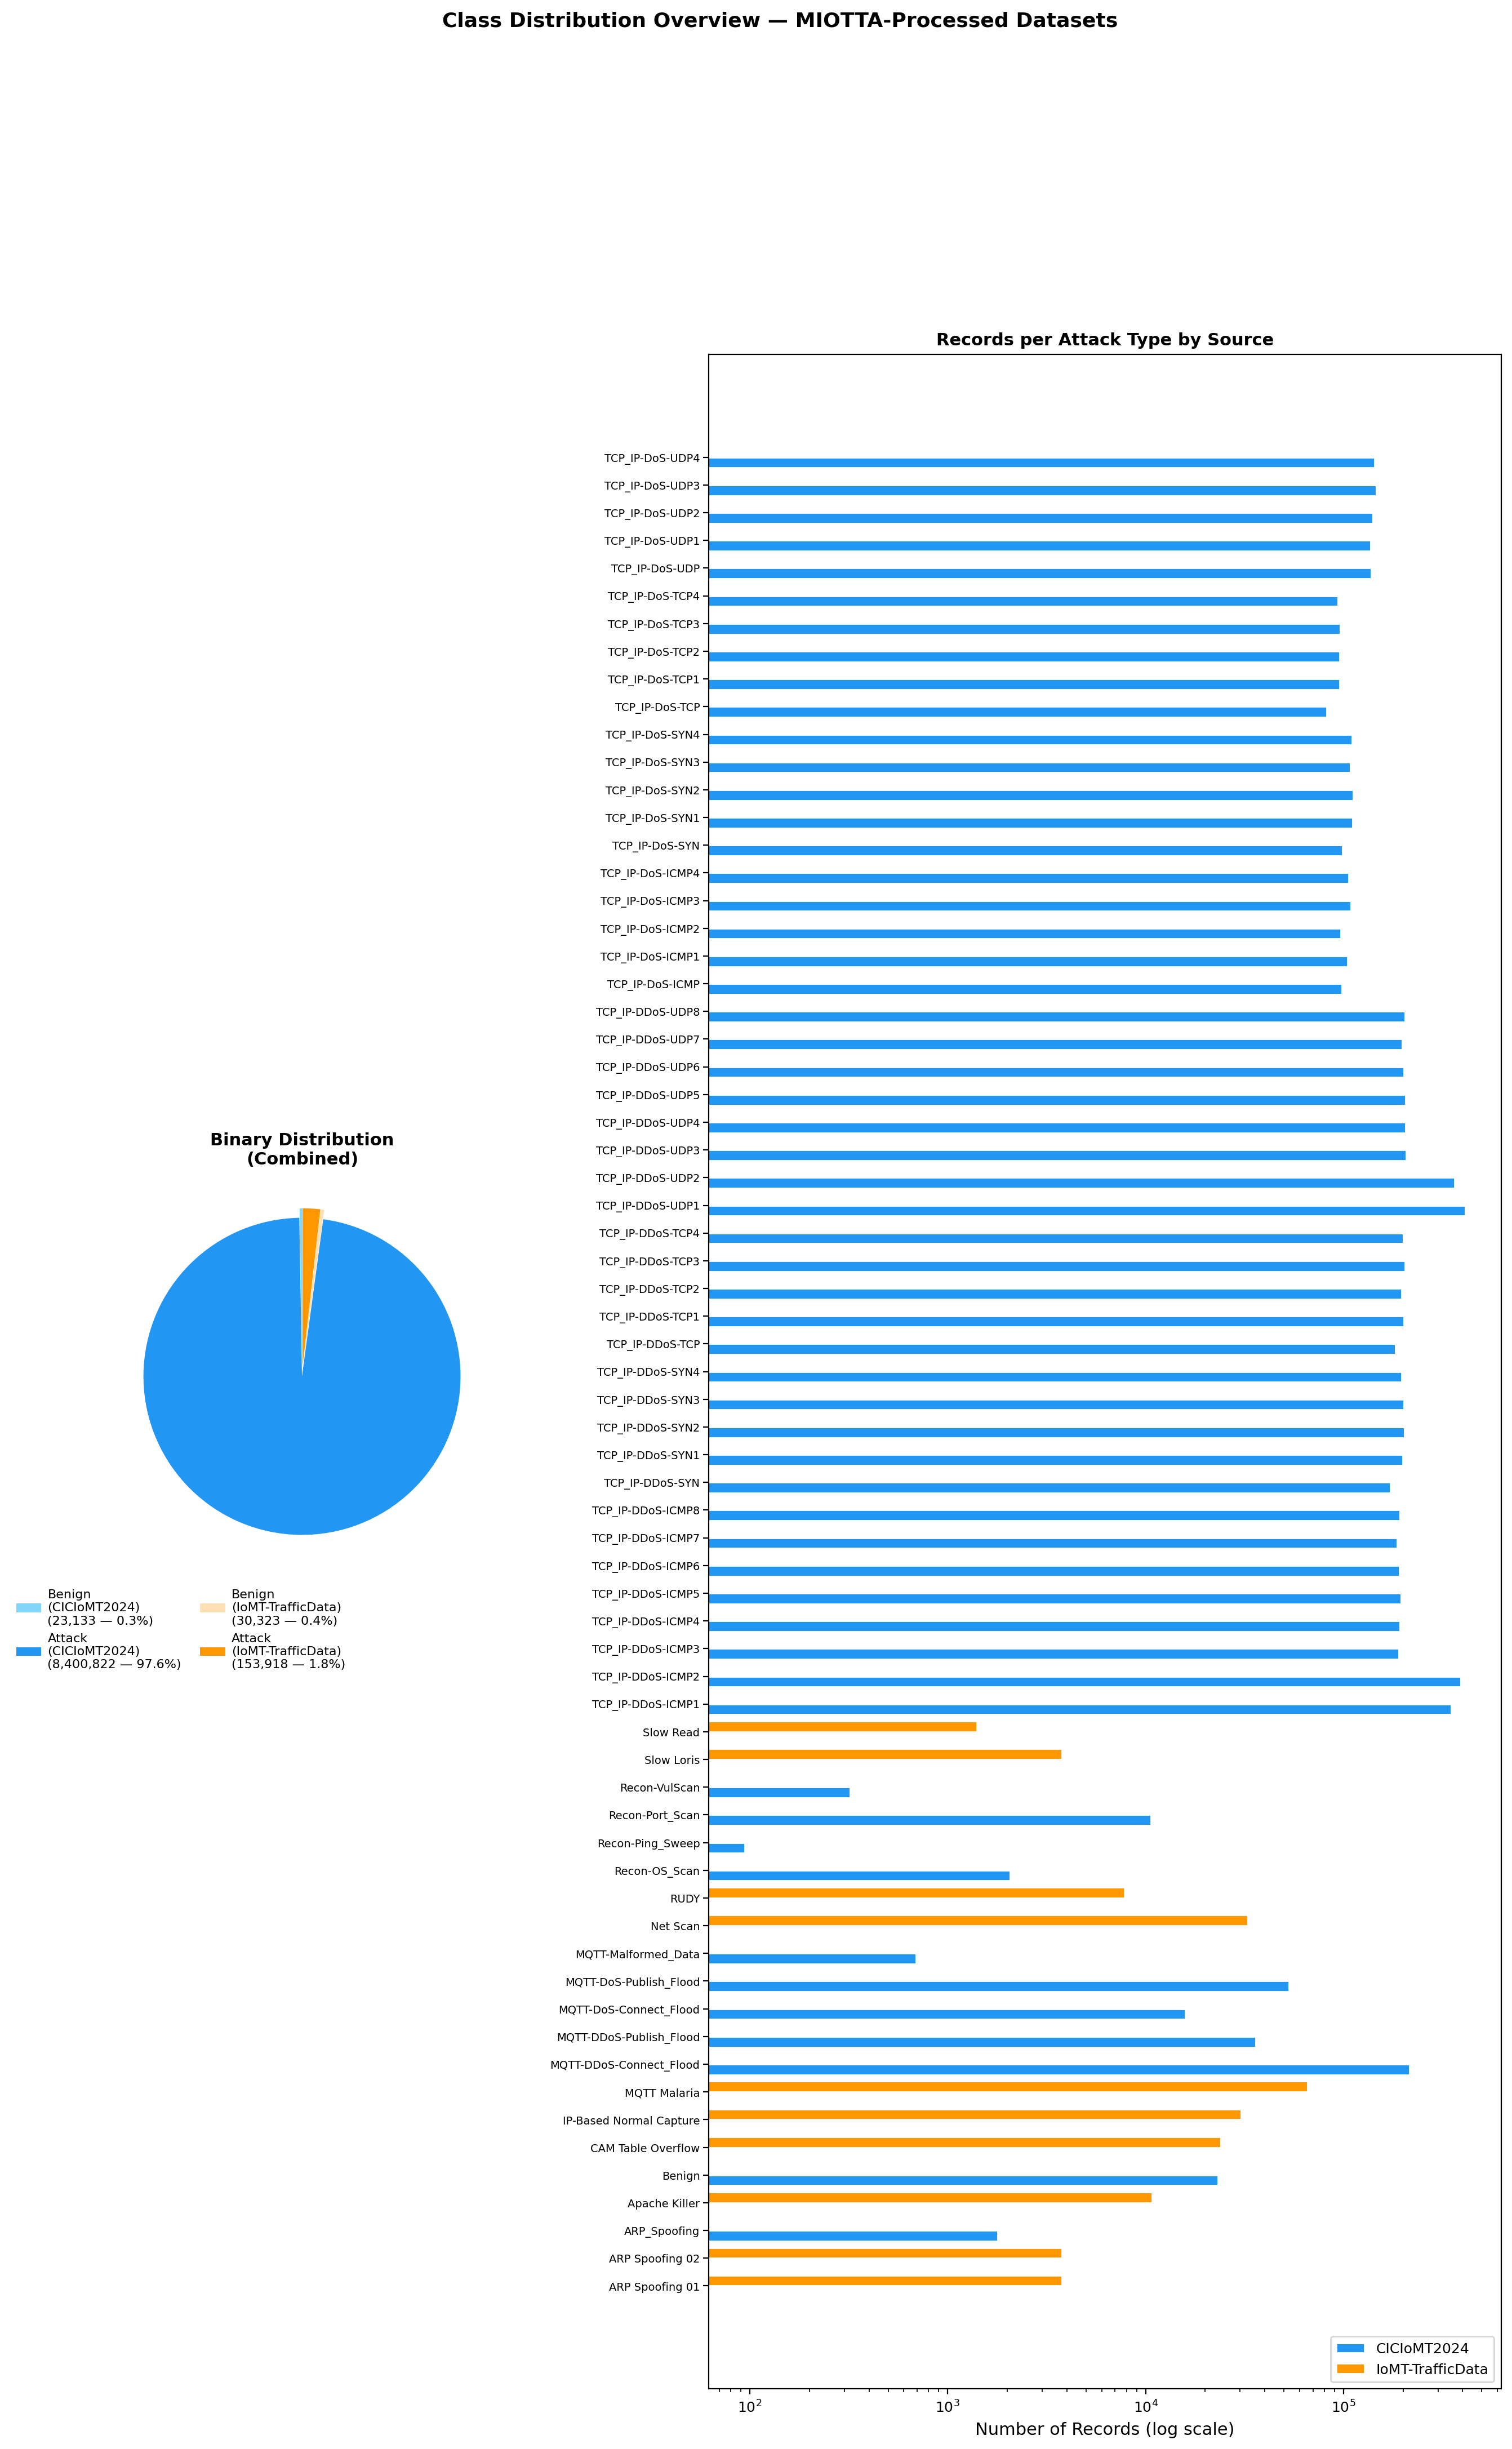
\includegraphics[height=0.85\textheight, keepaspectratio]{combined_class_distribution.png}
\caption{Class distribution overview of the two MIOTTA-processed datasets. Left: binary (benign vs. attack) composition showing the relative contribution of each dataset. Right: per-attack-type record counts by source dataset (logarithmic scale), illustrating the complementary attack coverage.}
\label{fig:combined-class-dist}
\end{figure}
\clearpage

% ══════════════════════════════════════════════════════════════════════════════
\section{Integration Pipeline Execution}
\label{sec:pipeline-execution}

This section documents the step-by-step execution of the integration pipeline, from label harmonization through to the production of the final unified dataset. Figure~\ref{fig:combined-class-dist} provides an overview of the class composition across the two datasets prior to integration.

\subsection{Label Harmonization Implementation}
\label{subsec:label-implementation}

The label harmonization stage applies the three-level labeling scheme defined in Section~\ref{sec:label-harmonization} through explicit mapping dictionaries maintained as configuration artifacts. Each original attack label is deterministically mapped to three harmonized levels: binary (\texttt{label\_binary}), category (\texttt{label\_category}), and fine-grained (\texttt{label\_fine}).

\paragraph{CICIoMT2024 Mapping.}
The CICIoMT2024 dataset contains 18 distinct attack types plus benign traffic. Table~\ref{tab:ciciomt-mapping} presents the complete mapping used in the final Phase~1 dataset. Attack labels are inferred from the MIOTTA output filenames and normalized by stripping numeric suffixes (e.g., \texttt{TCP\_IP-DDoS-ICMP1} through \texttt{TCP\_IP-DDoS-ICMP8} are collapsed to \texttt{TCP\_IP-DDoS-ICMP}). In this operational mapping, all MQTT-related attacks are grouped under the dedicated \texttt{MQTT} category to preserve protocol semantics for downstream model training and evaluation.

\begin{table}[htbp]
\centering
\caption{CICIoMT2024 label harmonization mapping used in Phase~1. The 19 original labels (including Benign) are mapped to 6 categories, including dedicated \texttt{MQTT}.}
\label{tab:ciciomt-mapping}
\small
\begin{tabularx}{\textwidth}{@{}l l l@{}}
\toprule
\textbf{Original Label (label\_fine)} & \textbf{Category} & \textbf{Binary} \\
\midrule
Benign & Benign & Benign \\
\addlinespace
TCP\_IP-DDoS-ICMP & DDoS & Attack \\
TCP\_IP-DDoS-UDP & DDoS & Attack \\
TCP\_IP-DDoS-SYN & DDoS & Attack \\
TCP\_IP-DDoS-TCP & DDoS & Attack \\
MQTT-DDoS-Connect\_Flood & MQTT & Attack \\
MQTT-DDoS-Publish\_Flood & MQTT & Attack \\
\addlinespace
TCP\_IP-DoS-UDP & DoS & Attack \\
TCP\_IP-DoS-SYN & DoS & Attack \\
TCP\_IP-DoS-ICMP & DoS & Attack \\
TCP\_IP-DoS-TCP & DoS & Attack \\
MQTT-DoS-Connect\_Flood & MQTT & Attack \\
MQTT-DoS-Publish\_Flood & MQTT & Attack \\
\addlinespace
Recon-Port\_Scan & Reconnaissance & Attack \\
Recon-OS\_Scan & Reconnaissance & Attack \\
Recon-VulScan & Reconnaissance & Attack \\
Recon-Ping\_Sweep & Reconnaissance & Attack \\
\addlinespace
ARP\_Spoofing & Spoofing & Attack \\
\addlinespace
MQTT-Malformed\_Data & MQTT & Attack \\
\bottomrule
\end{tabularx}
\end{table}

\paragraph{IoMT-TrafficData Mapping.}
The IoMT-TrafficData dataset uses descriptive filenames as attack labels. Table~\ref{tab:iomt-mapping} presents the mapping. Notably, two ARP Spoofing captures (variants 01 and 02) are consolidated into a single fine-grained label \texttt{ARP\_Spoofing}. In the dedicated MQTT mapping, \texttt{MQTT Malaria} is assigned to \texttt{MQTT}, while the remaining service-availability attacks (Apache Killer, CAM Table Overflow, SlowLoris, SlowRead, RUDY) remain in \texttt{DoS}.

\begin{table}[htbp]
\centering
\caption{IoMT-TrafficData label harmonization mapping used in Phase~1. The 10 original labels are mapped to 5 categories, including dedicated \texttt{MQTT}.}
\label{tab:iomt-mapping}
\small
\begin{tabularx}{\textwidth}{@{}l l l l@{}}
\toprule
\textbf{Original Label} & \textbf{Fine-Grained} & \textbf{Category} & \textbf{Binary} \\
\midrule
IP-Based Normal Capture & Benign & Benign & Benign \\
\addlinespace
MQTT Malaria & MQTT\_Malaria & MQTT & Attack \\
CAM Table Overflow & CAM\_Table\_Overflow & DoS & Attack \\
Apache Killer & Apache\_Killer & DoS & Attack \\
RUDY & RUDY & DoS & Attack \\
Slow Loris & SlowLoris & DoS & Attack \\
Slow Read & SlowRead & DoS & Attack \\
\addlinespace
Net Scan & Net\_Scan & Reconnaissance & Attack \\
\addlinespace
ARP Spoofing 01 & ARP\_Spoofing & Spoofing & Attack \\
ARP Spoofing 02 & ARP\_Spoofing & Spoofing & Attack \\
\bottomrule
\end{tabularx}
\end{table}

After harmonization, CICIoMT2024 spans 6 categories (DDoS, DoS, MQTT, Benign, Reconnaissance, Spoofing), while IoMT-TrafficData spans 5 categories (DoS, MQTT, Reconnaissance, Benign, Spoofing). The validation step confirmed that every original label was successfully mapped---no unmapped labels remained.

\subsection{Data Quality Treatment}
\label{subsec:quality-treatment}

The data quality assurance pipeline was applied to the unified dataset (8,608,196 rows, 73 features) in six sequential steps, as specified in Section~\ref{sec:quality}. Figure~\ref{fig:qa-impact} summarizes the aggregate impact.

\begin{figure}[htbp]
\centering
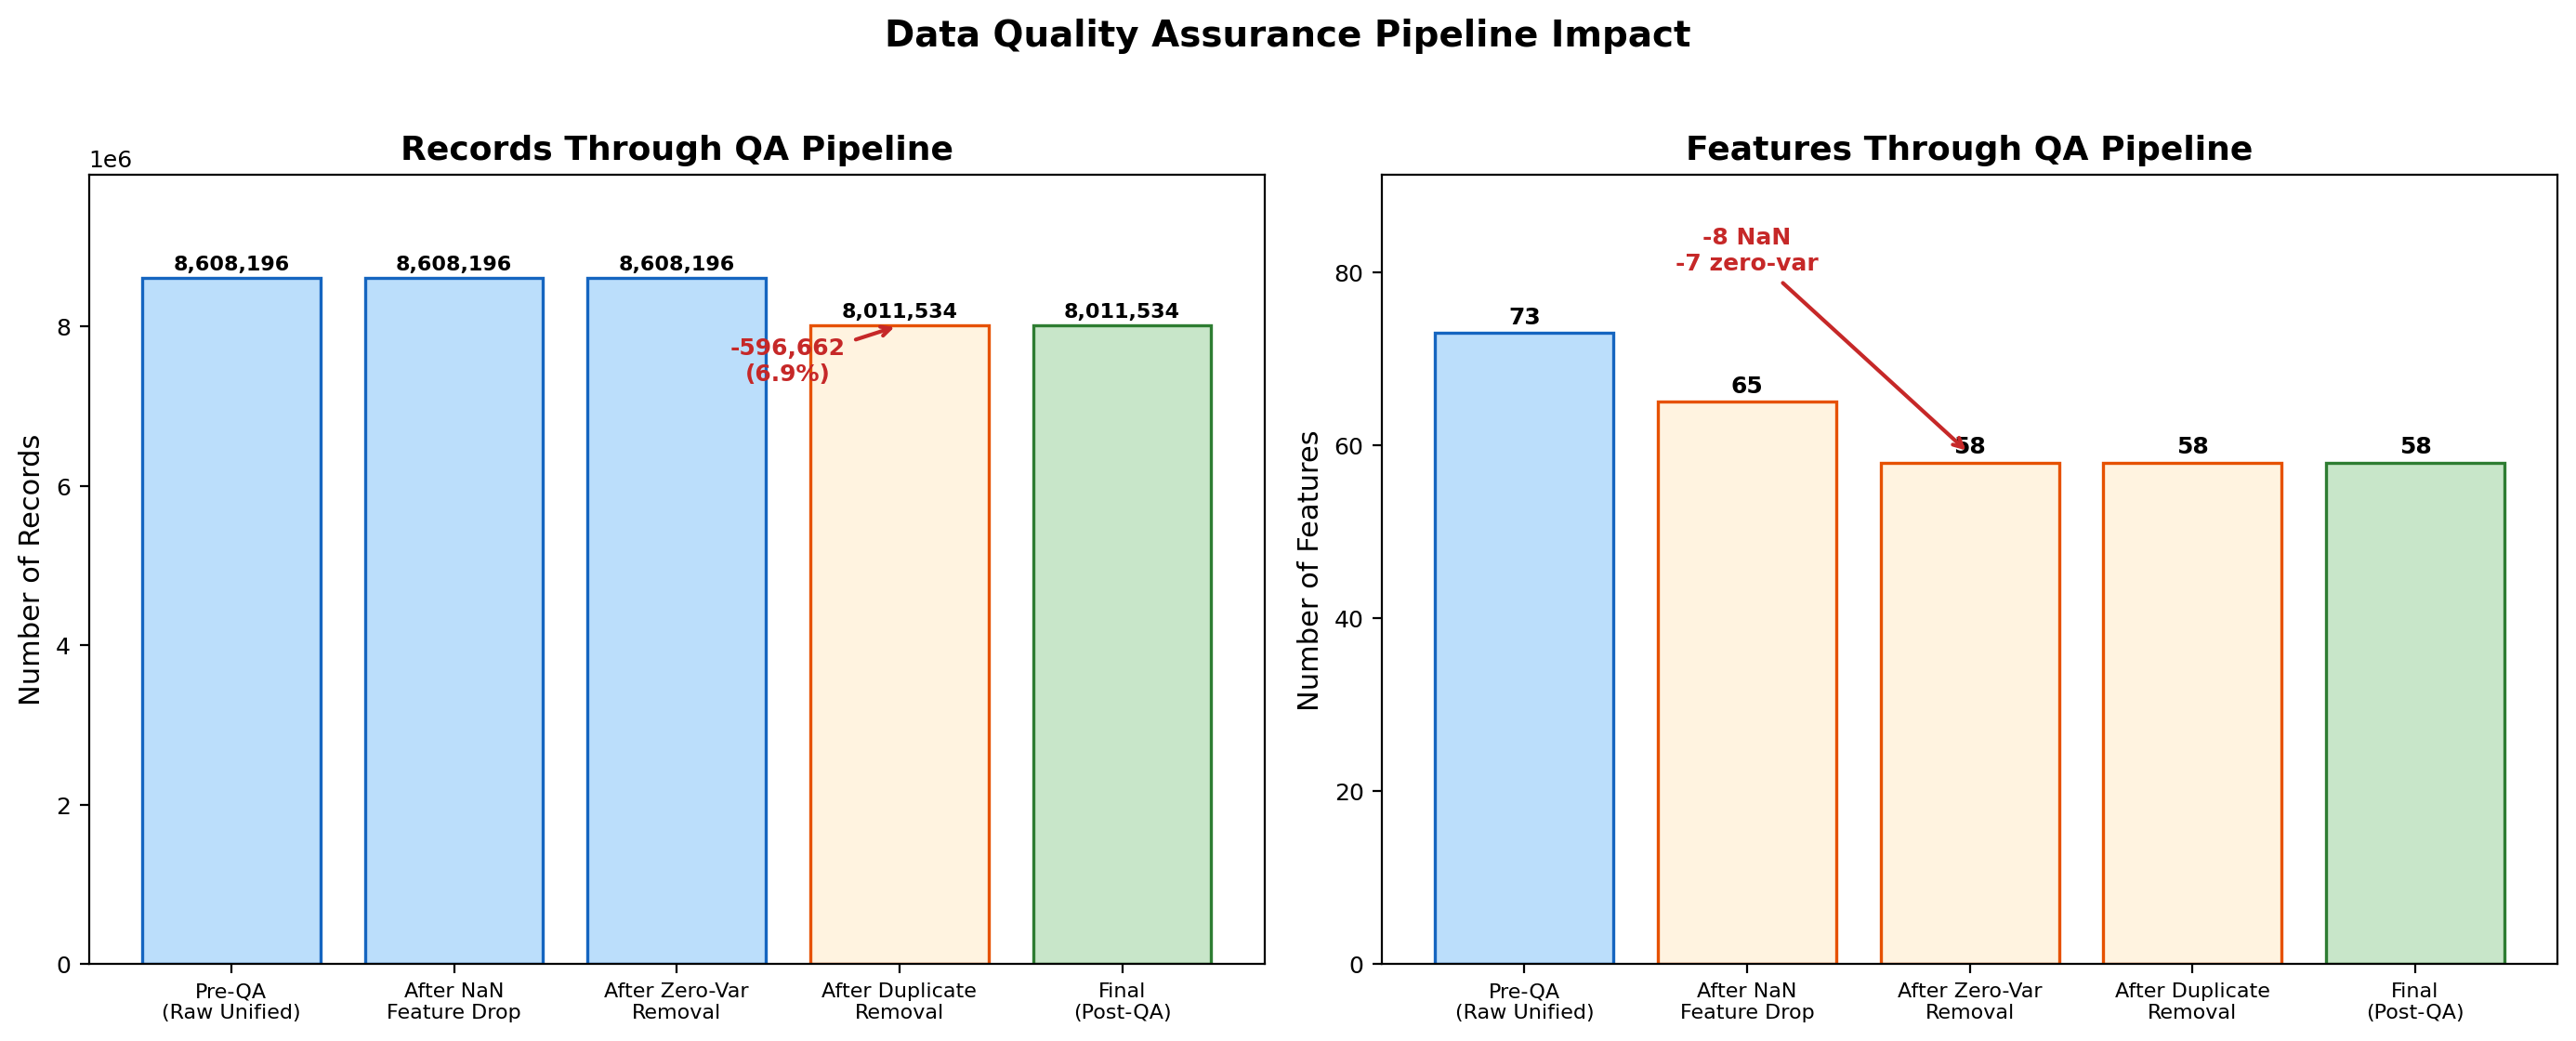
\includegraphics[width=\textwidth]{qa_impact_summary.png}
\caption{Impact of the data quality assurance pipeline on dataset dimensions. Left: record count reduction through duplicate removal. Right: feature reduction through high-NaN and zero-variance feature elimination.}
\label{fig:qa-impact}
\end{figure}

\paragraph{Step 1 --- Missing Value Treatment.}
Features with a NaN rate exceeding the 50\% threshold were dropped entirely. Eight TCP flag statistics met this criterion---\texttt{fin\_flag\_number}, \texttt{syn\_flag\_number}, \texttt{rst\_flag\_number}, \texttt{psh\_flag\_number}, \texttt{ack\_flag\_number}, \texttt{ece\_flag\_number}, \texttt{cwr\_flag\_number}, and \texttt{tcp\_flags\_ece}---all exhibiting 98.28\% missingness. This extreme rate is explained by the MIOTTA-NPT processing: these features count per-flag occurrences within a window, but when the window contains exclusively non-TCP traffic (UDP, ICMP, or ARP), no TCP flags exist and the values are recorded as NaN. Since 98.28\% of windows across both datasets lack these values, the features carry negligible discriminative information and their removal is justified. After dropping these 8 features, exactly 1 residual NaN value remained across the entire dataset, which was imputed with 0 following the protocol-absence pattern.

\paragraph{Step 2 --- Infinity Value Handling.}
A scan for $\pm\infty$ values found \textbf{zero infinity values} in any of the remaining 65 features. This indicates that the MIOTTA-NPT extraction tool handles edge cases (e.g., division by zero in rate computations) gracefully, producing NaN rather than infinity.

\paragraph{Step 3 --- Zero-Variance Feature Removal.}
Seven features exhibited exactly zero variance across the entire unified dataset and were removed: \texttt{DHCP}, \texttt{ARP}, \texttt{IPV4}, \texttt{LLC}, \texttt{Drate}, \texttt{Fwd\_Data\_Pkts\_Tot}, and \texttt{Bwd\_Data\_Pkts\_Tot}. These constant-valued features carry no discriminative information for classification. Their presence reflects either protocol indicators that never trigger in the IoMT traffic or aggregation counters that are always zero in the combined mode.

\paragraph{Step 4 --- Near-Zero-Variance Detection.}
Four additional features were flagged as having near-zero variance (below $10^{-8}$): \texttt{IGMP}, \texttt{Fwd\_IAT}, \texttt{Bwd\_IAT}, and \texttt{Flow\_IAT}. These were \textit{not} removed, as they may still carry useful information for specific attack categories, but they were recorded in the pipeline metadata for consideration during model evaluation.

\paragraph{Step 5 --- Duplicate Removal.}
Exact duplicate detection, applied on feature columns only (excluding metadata and label columns), identified and removed \textbf{596,662 duplicate rows} (6.93\% of the pre-QA dataset). Duplicates arise from the window-based aggregation methodology: consecutive windows of identical packet patterns produce identical feature vectors, particularly common in DDoS flood attacks where sustained high-volume traffic creates highly repetitive patterns. The first occurrence of each unique row was retained.

\paragraph{Step 6 --- Type Consistency.}
All 58 remaining feature columns were cast from their original \texttt{float64} type to \texttt{float32}, halving memory requirements while preserving sufficient numerical precision for ML training. This standardization ensures that all features use a uniform data type regardless of their source dataset.

\subsection{Dataset Concatenation and Source Attribution}
\label{subsec:concatenation}

Prior to quality assurance, the two harmonized datasets were concatenated into a single unified DataFrame. The concatenation was performed using a simple vertical stack (\texttt{pd.concat}), made possible by the identical feature schema guaranteed by MIOTTA-NPT processing.

Each record retains three provenance columns: \texttt{source\_dataset} identifies the originating dataset (\texttt{CICIoMT2024} or \texttt{IoMT-TrafficData}), \texttt{source\_file} records the specific MIOTTA output CSV file, and \texttt{attack\_type} preserves the original label as inferred from the filename. These columns enable cross-domain evaluation and per-source performance disaggregation, as discussed in Section~\ref{sec:provenance}.

The pre-QA unified dataset comprised 8,608,196 records (8,423,955 from CICIoMT2024, representing 97.86\%, and 184,241 from IoMT-TrafficData, representing 2.14\%) with 73 features and 7 metadata/label columns (80 columns total). After the complete QA pipeline, the final unified dataset contains \textbf{8,011,534 records} across \textbf{58 features}, plus the label and metadata columns.

\subsection{Feature Scaling}
\label{subsec:scaling-execution}

Feature scaling was applied using \textbf{standardization} ($z$-score normalization), transforming each feature to zero mean and unit variance. To prevent data leakage, the scaling parameters (per-feature mean and standard deviation) were computed exclusively on the training partition and then applied identically to the validation and test partitions.

The implementation uses scikit-learn's \texttt{StandardScaler}, fitted on the training set's 58 feature columns. Post-scaling verification confirmed that the training set achieves a mean $\approx 0.000000$ and standard deviation $\approx 1.000000$ across all features, as expected. The validation and test sets exhibit means and standard deviations very close to---but not exactly---0 and 1, which is the correct behavior: slight deviations confirm that no information from these partitions leaked into the scaling parameters.

The fitted scaler object is persisted as a \texttt{joblib} artifact (\texttt{scaler.joblib}), enabling its reuse during model inference to ensure that new data undergoes identical preprocessing.

\subsection{Stratified Splitting}
\label{subsec:splitting-execution}

The unified dataset was partitioned into training, validation, and test sets using scikit-learn's \texttt{train\_test\_split} with stratification on the composite key \texttt{label\_category} $\times$ \texttt{source\_dataset}. This dual stratification ensures that both the attack category distribution and the source dataset proportions are preserved in each partition, preventing any partition from accidentally excluding rare attack types or under-representing a source dataset.

The split was performed in two stages: first, 70\% of the data was allocated to the training set and 30\% to a temporary hold-out; then, the hold-out was divided equally into 15\% validation and 15\% test. Table~\ref{tab:split-sizes} presents the resulting partition sizes.

\begin{table}[htbp]
\centering
\caption{Stratified split sizes for the Phase~1 unified dataset.}
\label{tab:split-sizes}
\small
\begin{tabular}{@{}l r r r r@{}}
\toprule
\textbf{Partition} & \textbf{Records} & \textbf{\%} & \textbf{CICIoMT2024} & \textbf{IoMT-TrafficData} \\
\midrule
Train & 5,608,073 & 70.0\% & 5,479,105 (97.70\%) & 128,968 (2.30\%) \\
Validation & 1,201,730 & 15.0\% & 1,174,094 (97.70\%) & 27,636 (2.30\%) \\
Test & 1,201,731 & 15.0\% & 1,174,094 (97.70\%) & 27,637 (2.30\%) \\
\midrule
\textbf{Total} & \textbf{8,011,534} & \textbf{100\%} & \textbf{7,827,293} & \textbf{184,241} \\
\bottomrule
\end{tabular}
\end{table}

Figure~\ref{fig:split-verification} confirms that stratification successfully preserves both category and source proportions across all three partitions for the dedicated MQTT mapping. Category proportions remain near-identical across train/validation/test (DDoS: 67.01\%, DoS: 26.82\%, MQTT: 4.82\%, Benign: 0.67\%, Reconnaissance: 0.57\%, Spoofing: 0.12\%), while source proportions are preserved to within $\pm0.01\%$. This level of consistency is essential for ensuring that model evaluation metrics are not confounded by partition-level distribution differences.

\begin{figure}[htbp]
\centering
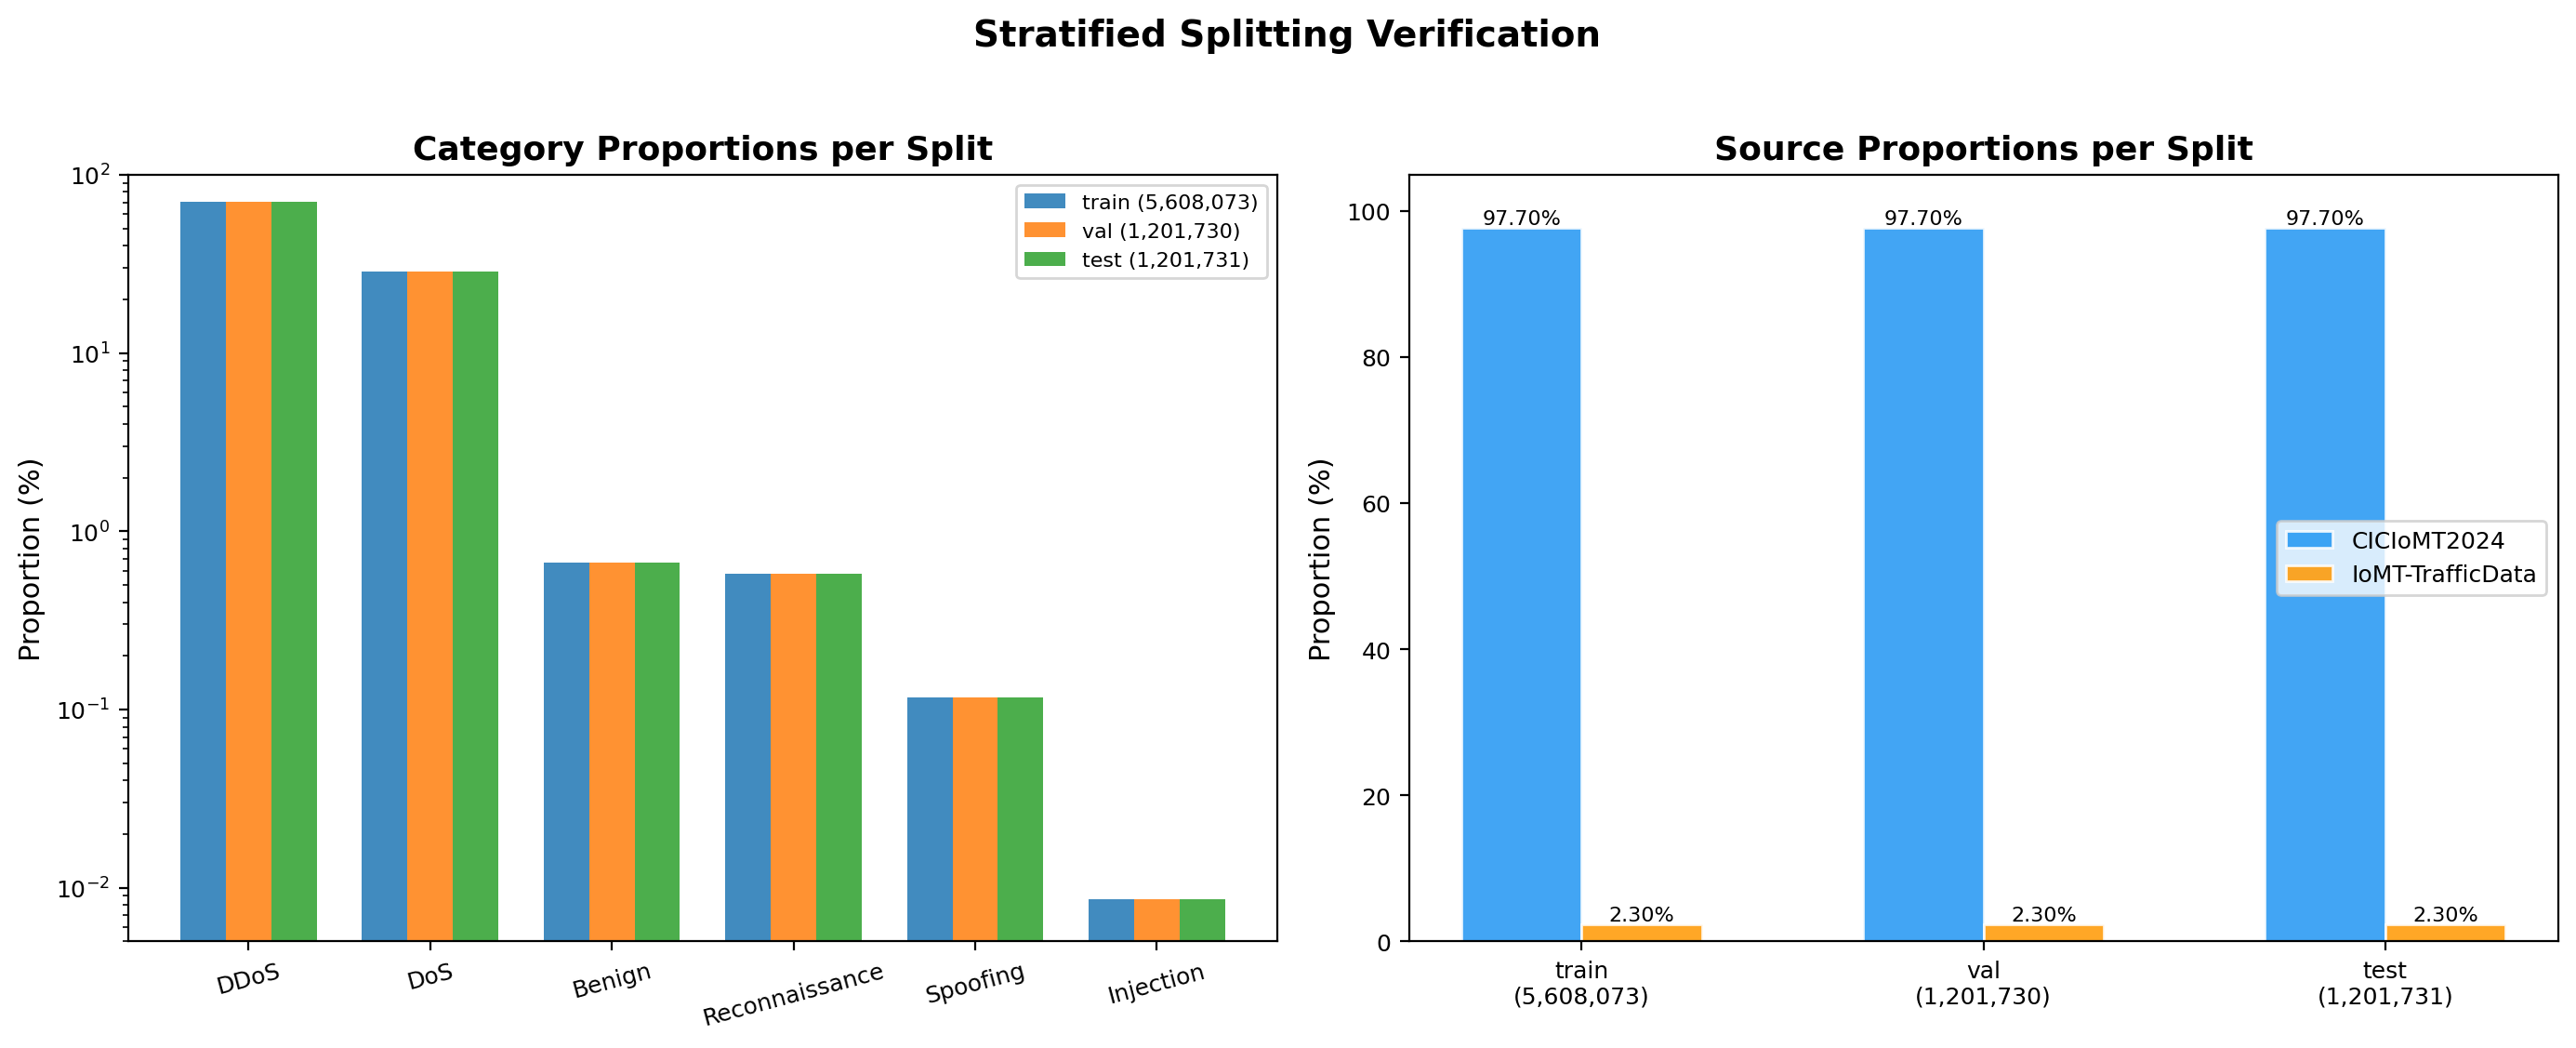
\includegraphics[width=\textwidth]{split_verification.png}
\caption{Verification of stratified splitting. Left: category proportions per partition (logarithmic scale). Right: source dataset proportions per partition. The near-identical proportions confirm successful stratification.}
\label{fig:split-verification}
\end{figure}

% ══════════════════════════════════════════════════════════════════════════════
\section{Unified Dataset Description}
\label{sec:unified-description}

The Phase~1 integration pipeline produces a unified IoMT intrusion detection dataset that combines traffic from two complementary IoMT environments into an ML-ready resource. Following supervisor guidance, all subsequent experiments in this thesis adopt the dedicated MQTT category mapping at Level-2, where all MQTT-related attacks are grouped under \texttt{MQTT}. This section characterizes the final dataset used for model development.

\subsection{Dataset Overview}
\label{subsec:dataset-overview}

The final unified dataset comprises \textbf{8,011,534 records} described by \textbf{58 numeric features}, partitioned into training (5,608,073), validation (1,201,730), and test (1,201,731) sets. All features are standardized with \texttt{StandardScaler} using train-only fitting (fit on train; transform on train/validation/test), cast to \texttt{float32} for memory efficiency, and verified to contain no missing, infinite, or constant-valued entries.

\subsection{Label Distributions}
\label{subsec:label-distributions}

The three-level labeling scheme provides classification targets at different granularities:

\begin{itemize}
    \item \textbf{Binary level}: 99.33\% of records are labeled as \texttt{Attack} and 0.67\% as \texttt{Benign}, reflecting the attack-heavy nature of the source datasets.

    \item \textbf{Category level}: Six categories are present, with the distribution shown in Figure~\ref{fig:unified-categories}. DDoS dominates with 67.01\% of records, followed by DoS (26.82\%), MQTT (4.82\%), Benign (0.67\%), Reconnaissance (0.57\%), and Spoofing (0.12\%). The maximum-to-minimum ratio is approximately 575:1 (DDoS vs.\ Spoofing), indicating substantial class imbalance that must be addressed during model training.

    \item \textbf{Fine-grained level}: 26 distinct attack types are present, spanning both datasets. The four most common types---\texttt{TCP\_IP-DDoS-ICMP} (21.71\%), \texttt{TCP\_IP-DDoS-UDP} (21.45\%), \texttt{TCP\_IP-DDoS-SYN} (12.09\%), and \texttt{TCP\_IP-DDoS-TCP} (11.76\%)---together account for 67\% of all records. The rarest types, \texttt{Recon-Ping\_Sweep} (94 records) and \texttt{Recon-VulScan} (322 records), constitute less than 0.005\% of the dataset.
\end{itemize}

\begin{figure}[htbp]
\centering
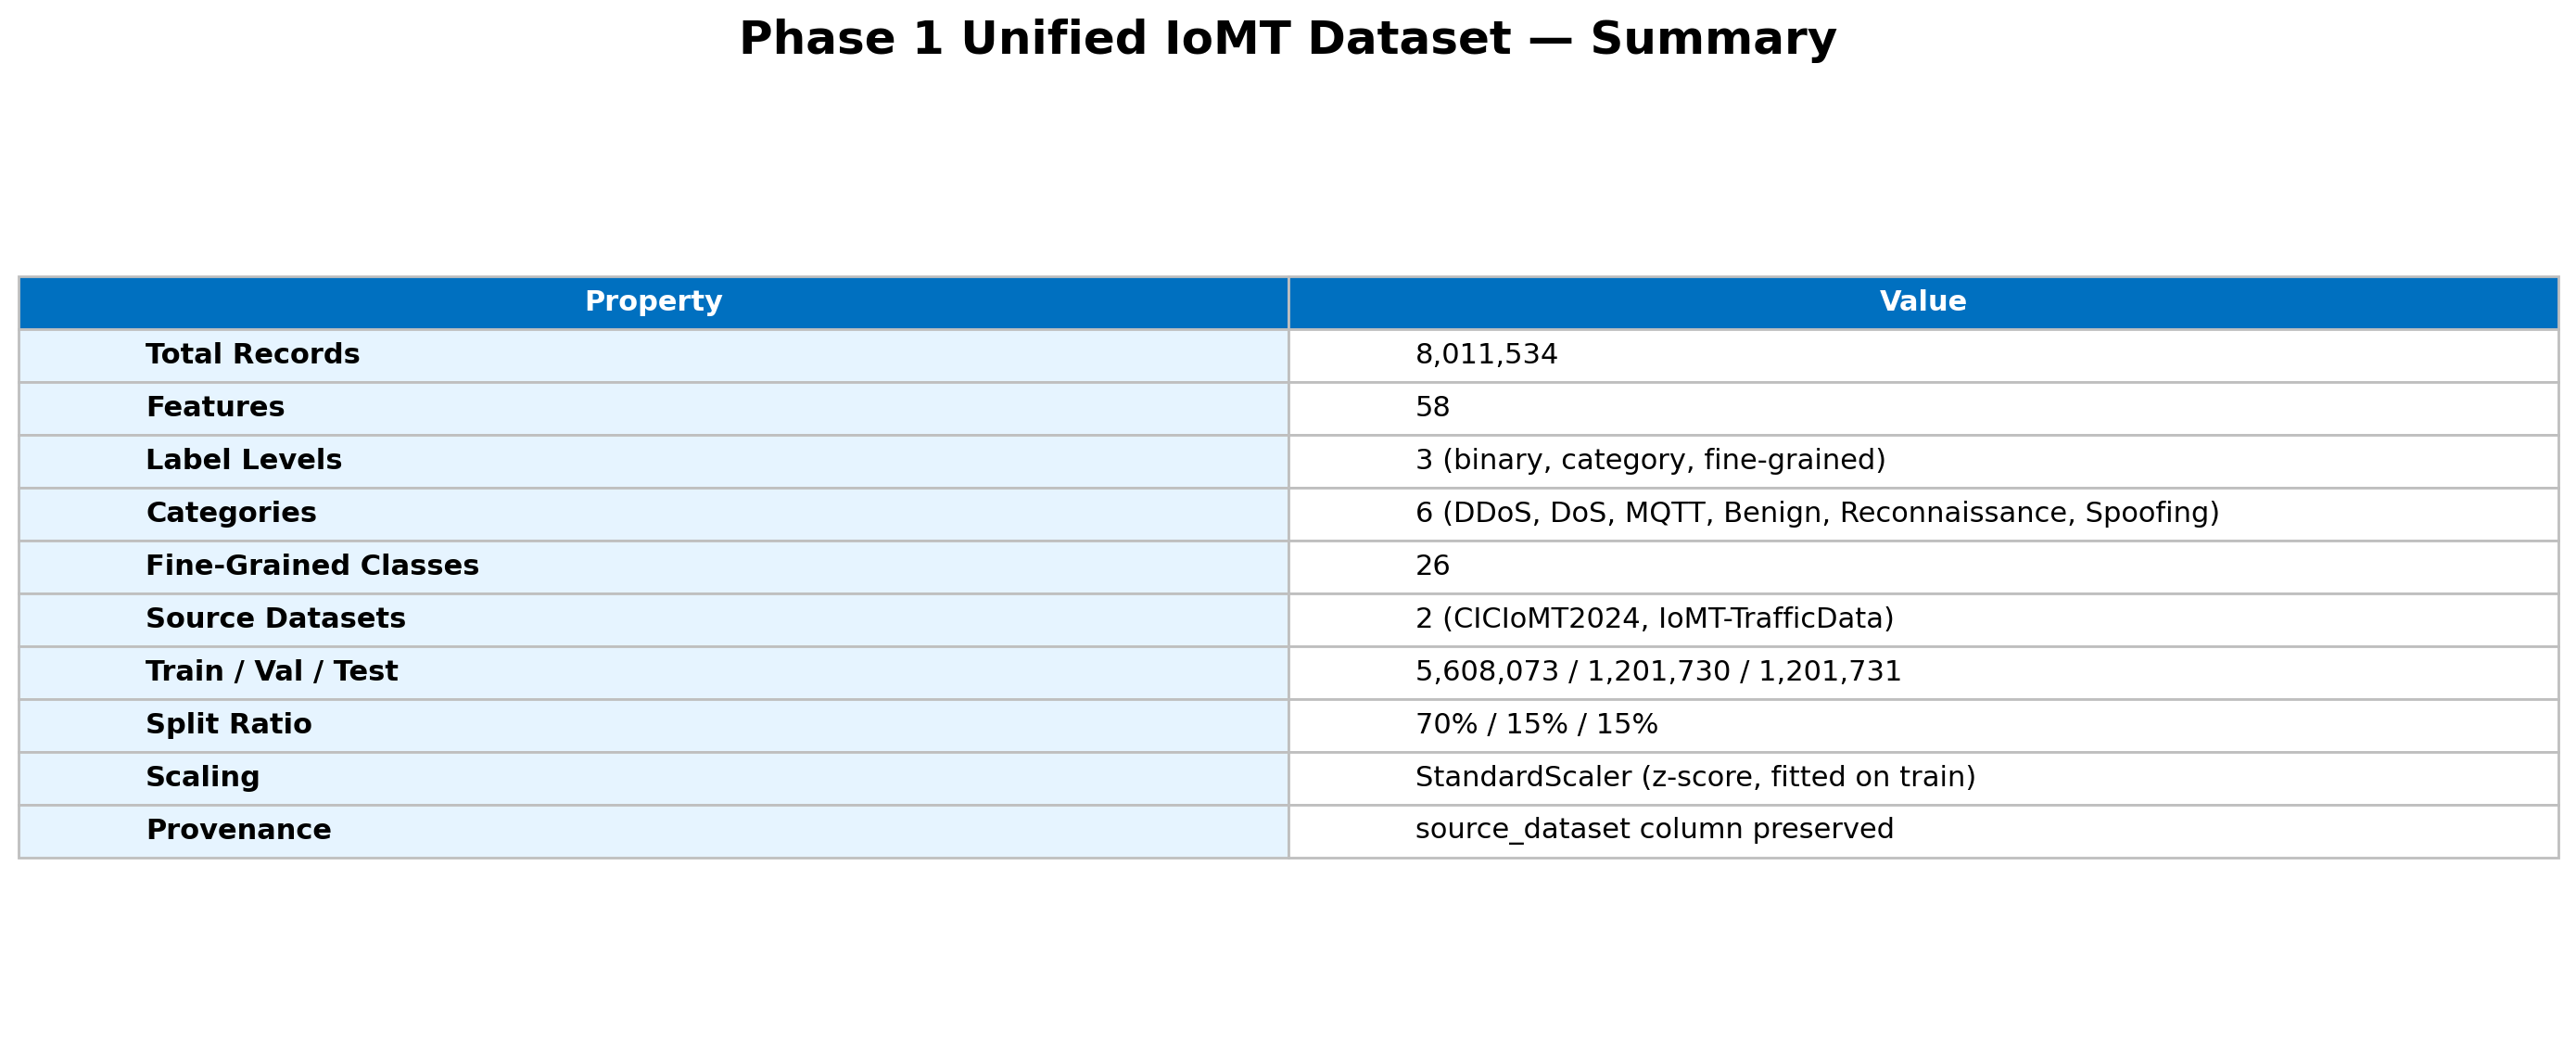
\includegraphics[width=0.85\textwidth]{unified_dataset_summary.png}
\caption{Summary of the final Phase~1 unified IoMT intrusion detection dataset used for model development (dedicated MQTT mapping).}
\label{fig:unified-summary}
\end{figure}

\begin{figure}[htbp]
\centering
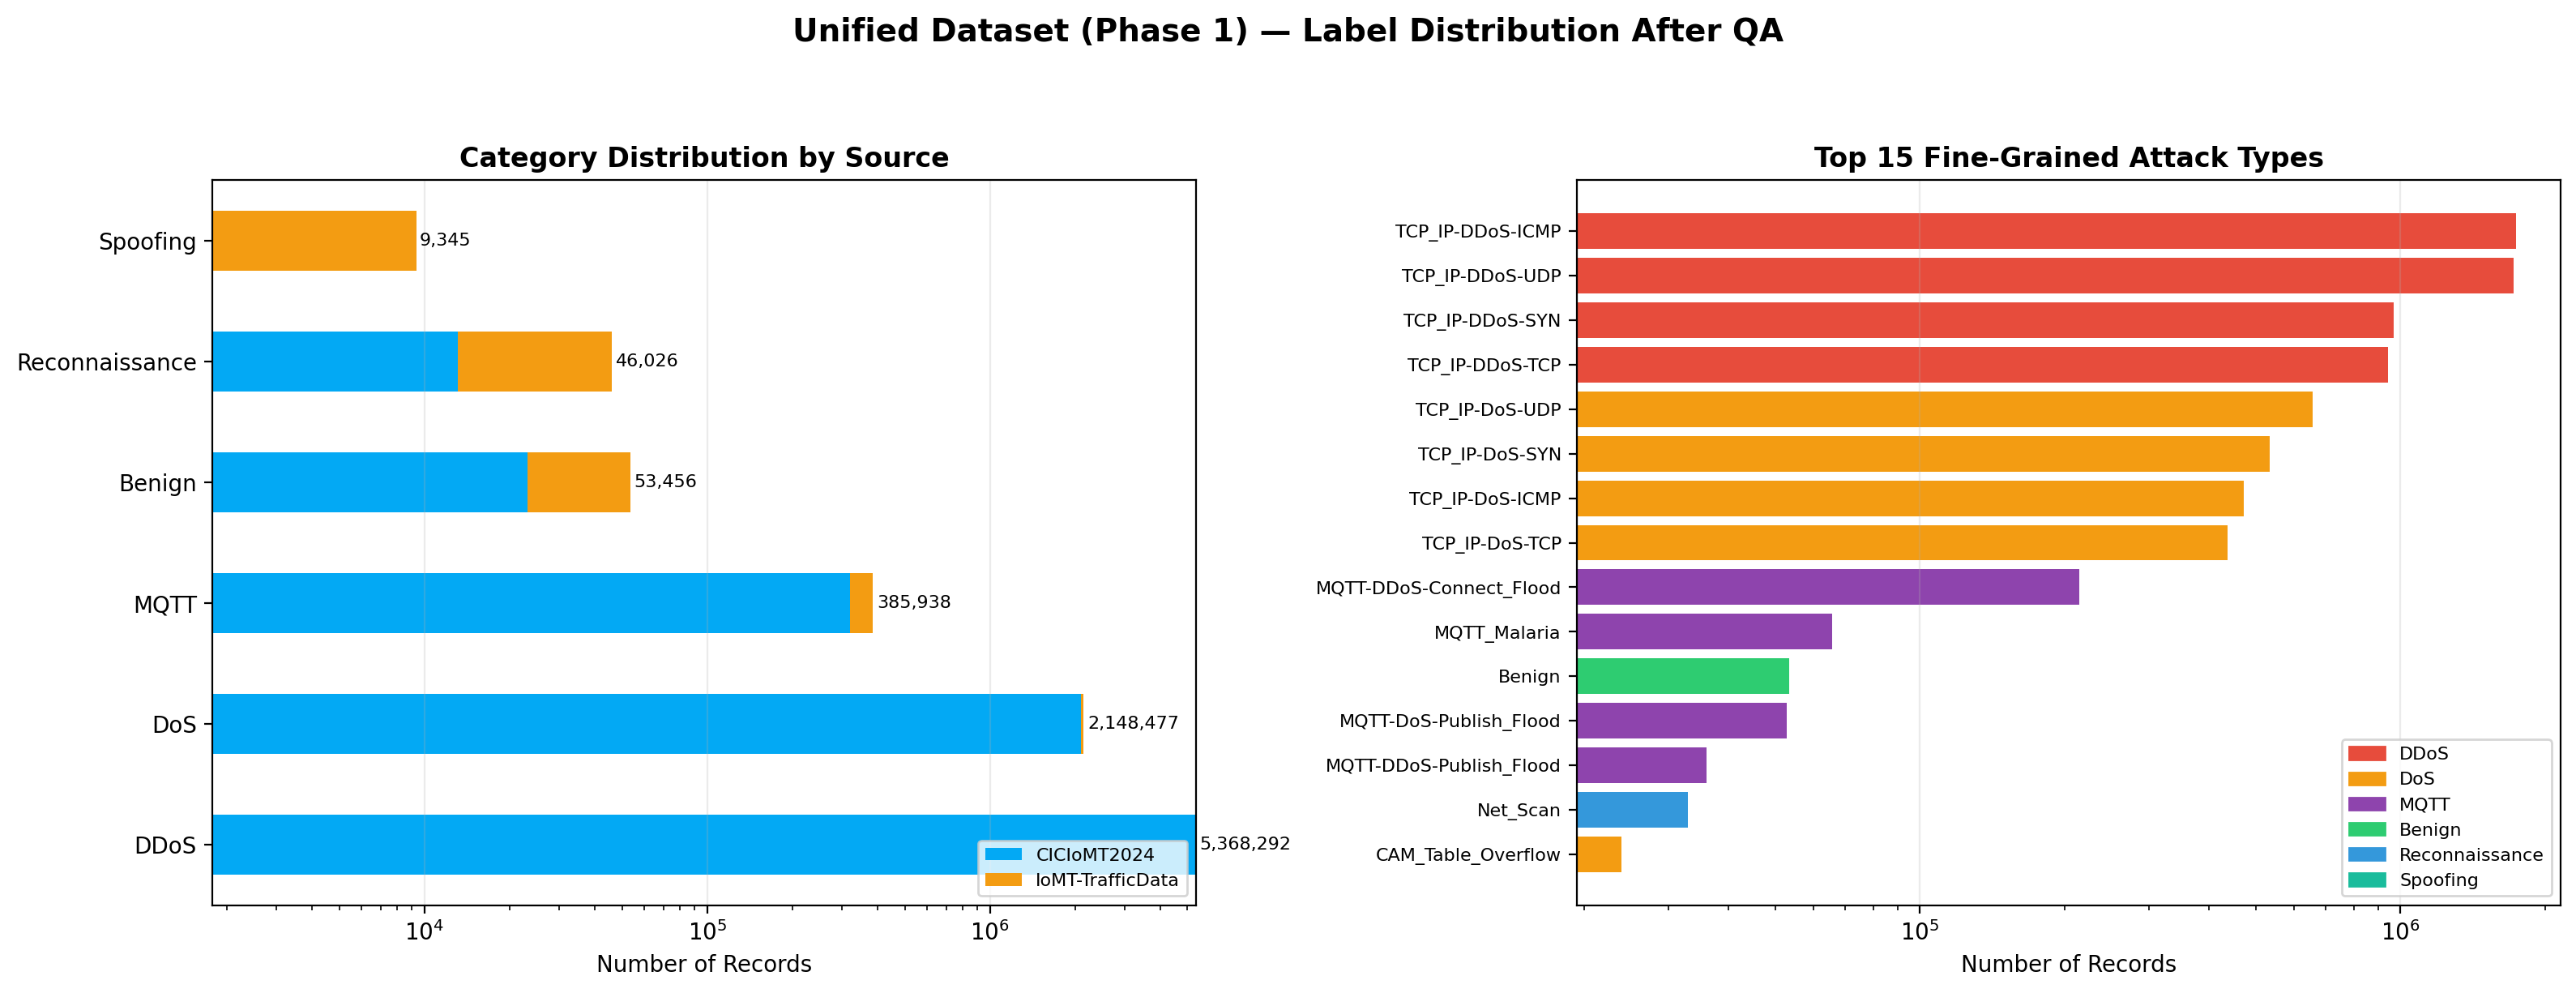
\includegraphics[width=\textwidth]{unified_category_distribution.png}
\caption{Label distribution in the final Phase~1 unified dataset (dedicated MQTT mapping). Left: category-level distribution decomposed by source dataset. Right: the 15 most frequent fine-grained attack types, color-coded by category.}
\label{fig:unified-categories}
\end{figure}

\subsection{Category-Mapping Rationale}
\label{subsec:mqtt-variant}

The dedicated MQTT mapping was selected as the operational taxonomy because the subsequent objective is protocol-aware model evaluation. Concretely, for CICIoMT2024, \texttt{MQTT-DDoS-Connect\_Flood}, \texttt{MQTT-DDoS-Publish\_Flood}, \texttt{MQTT-DoS-Connect\_Flood}, \texttt{MQTT-DoS-Publish\_Flood}, and \texttt{MQTT-Malformed\_Data} are mapped to \texttt{MQTT}; for IoMT-TrafficData, \texttt{MQTT Malaria} is also mapped to \texttt{MQTT}. All other processing stages (quality treatment, stratified splitting, train-only scaler fitting, and export) remain unchanged.

The resulting post-QA category distribution (8,011,534 records, matching the exported CSV splits) is: DDoS 67.01\%, DoS 26.82\%, MQTT 4.82\%, Benign 0.67\%, Reconnaissance 0.57\%, and Spoofing 0.12\%.

\subsection{Cross-Dataset Complementarity}
\label{subsec:complementarity}

A key design objective of the integration was to achieve complementary attack coverage. The unified dataset fulfills this objective: CICIoMT2024 contributes 97.70\% of the records and provides coverage of DDoS, DoS, MQTT, Reconnaissance, and Spoofing categories, while IoMT-TrafficData contributes 2.30\% and introduces 6 unique fine-grained attack types not present in CICIoMT2024---Apache\_Killer, CAM\_Table\_Overflow, MQTT\_Malaria, RUDY, SlowLoris, and SlowRead---covering both \texttt{DoS} and \texttt{MQTT} protocol-oriented behaviors.

Two fine-grained labels appear in both datasets: \texttt{Benign} and \texttt{ARP\_Spoofing}, enabling direct cross-dataset comparison for these specific traffic types. The shared \texttt{ARP\_Spoofing} label (1,782 records from CICIoMT2024, 7,563 from IoMT-TrafficData) is particularly valuable for assessing whether models can generalize the detection of the same attack across different network environments.

\subsection{Storage and Access}
\label{subsec:storage}

The final dataset used in this thesis is stored in \texttt{data/processed/phase1\_iomt\_unified\_mqtt\_category/}, containing the following artifacts:

\begin{itemize}
    \item \texttt{train.csv}, \texttt{val.csv}, \texttt{test.csv}: Scaled data partitions.
    \item \texttt{scaler.joblib}: Fitted \texttt{StandardScaler} object for inference-time preprocessing.
    \item \texttt{metadata.joblib}: Pipeline metadata including the final feature list, near-zero-variance features, and split sizes.
\end{itemize}

The total storage footprint is approximately 6.4~GB in CSV format. Each CSV file contains the 58 scaled features, the three label columns (\texttt{label\_binary}, \texttt{label\_category}, \texttt{label\_fine}), and the provenance columns (\texttt{source\_dataset}, \texttt{source\_file}, \texttt{attack\_type}, \texttt{attack\_group}).

% ══════════════════════════════════════════════════════════════════════════════
\section{Chapter Summary}
\label{sec:execution-summary}

This chapter documented the complete development and execution of the Phase~1 integration pipeline, progressing from exploratory analysis through to the production of unified IoMT intrusion detection datasets. The key contributions and findings of this chapter are:

\begin{enumerate}
    \item \textbf{Exploratory analysis} of three datasets (CICIoMT2024, IoMT-TrafficData, CICIoT2023) revealed fundamental structural incompatibilities in their original feature representations---45, 101, and 47 features respectively, extracted using different tools---confirming the necessity of MIOTTA-NPT for feature standardization.

    \item \textbf{MIOTTA-NPT processing} produced identical 73-feature representations for CICIoMT2024 (8,423,955 records) and IoMT-TrafficData (184,241 records), verified through empirical column-level comparison.

    \item \textbf{Label harmonization} mapped 19 original CICIoMT2024 labels and 10 original IoMT-TrafficData labels into a consistent three-level scheme (binary, category, fine-grained), with dedicated \texttt{MQTT} as the operational Level-2 category space used for all subsequent model development.

    \item \textbf{Data quality assurance} reduced the feature space from 73 to 58 features (removing 8~high-NaN and 7~zero-variance features) and eliminated 596,662 duplicate records (6.93\%), yielding a clean dataset of 8,011,534 records.

    \item \textbf{Stratified splitting} with dual stratification on category and source produced balanced train/validation/test partitions (70/15/15\%) with virtually identical category and source proportions across all three partitions.

    \item \textbf{Feature scaling} using StandardScaler fitted exclusively on the training partition prevents data leakage while ensuring normalized feature ranges for ML model training.
\end{enumerate}

The resulting unified dataset is ready for training and evaluating intrusion detection models in the next stage of this thesis. The pipeline's modular design facilitates extension in Phase~2 to incorporate CICIoT2023, broadening attack coverage to include Mirai botnet, web-based, and brute-force attacks while preserving the same reproducible preprocessing backbone.
